\documentclass[12pt, a4paper]{report}
\usepackage[utf8x]{inputenc}
\usepackage[T1]{fontenc}
\usepackage[hungarian]{babel}
\usepackage{amsmath}
\usepackage{amsfonts}
\usepackage{amssymb}
\usepackage{amsthm}
\usepackage{ccfonts}
\usepackage[euler-digits,euler-hat-accent]{eulervm}
\usepackage{graphicx}
\usepackage{ae}
\usepackage[margin=2cm]{geometry}
\usepackage{hyperref}
\usepackage{minted}
\usepackage[parfill]{parskip}
\usepackage{enumitem}

\makeatletter

\graphicspath{ {./images/} }

\newcommand{\f}[1]{\texttt{#1}}
\newcommand{\ff}[1]{\textbf{\texttt{#1}}}
\newcommand{\bb}[1]{\textbf{#1}}

\newminted[antlr4code]{"../pygments/Antlr4Lexer.py":Antlr4Lexer -x}{tabsize=2,fontsize=\footnotesize,baselinestretch=0.7,linenos=false,frame=single,breaklines=true,breakanywhere=true,style=sb}

\newmintedfile[metafile]{"../pygments/MetaLexer.py":MetaLexer -x}{tabsize=2,fontsize=\footnotesize,baselinestretch=0.7,linenos=false,frame=single,breaklines=true,breakanywhere=true,style=sb}
\newminted[mmcode]{"../pygments/MetaLexer.py":MetaLexer -x}{tabsize=2,fontsize=\footnotesize,baselinestretch=0.7,linenos=false,frame=single,breaklines=true,breakanywhere=true,style=sb}

\newminted[mgencode]{"../pygments/MGenLexer.py":MetaGeneratorLexer -x}{tabsize=2,fontsize=\footnotesize,baselinestretch=0.7,linenos=false,frame=single,breaklines=true,breakanywhere=true,style=sb}

\newminted{c}{tabsize=2,fontsize=\footnotesize,baselinestretch=0.7,linenos=false,frame=single,breaklines=true,breakanywhere=true}
\usemintedstyle[c]{vs}

\newminted{java}{tabsize=2,fontsize=\footnotesize,baselinestretch=0.7,linenos=false,frame=single,breaklines=true,breakanywhere=true}
\usemintedstyle[java]{vs}

\newminted{csharp}{tabsize=2,fontsize=\footnotesize,baselinestretch=0.7,linenos=false,frame=single,breaklines=true,breakanywhere=true,style=sb}

\newminted{text}{tabsize=2,fontsize=\footnotesize,baselinestretch=0.7,linenos=false,frame=single,breaklines=true,breakanywhere=true}

\setitemize{noitemsep,topsep=0pt,parsep=0pt,partopsep=0pt}


% Title Page
\title{MetaDslx keretrendszer}
\author{Dr. Simon Balázs}
\date{\today}


\begin{document}
\maketitle

\tableofcontents

\chapter{Bevezetés}

A MetaDslx keretrendszer célja, hogy megkönnyítse szakterület-specifikus nyelvek (DSL) kifejlesztését.

Egy szöveges DSL feldolgozása a fordítással kezdődik. A fordító értelmezi a kód szintaktikáját és jelentését, majd ha minden rendben van, akkor egy modellt épít, amely a DSL kódban leírt dolgokat reprezentálja. A modellt ezután kódgenerátorok járják be, és elkészítik a kimeneti generált kódot:

\begin{center}\includegraphics[trim=120 20 120 70,clip,width=\textwidth,page=14]{Images.pdf}\end{center}

Ahhoz hogy ezek a lépések működjenek, definiálnunk kell a felépítendő modell leírását, vagyis metamodelljét. Ezt egy .mm kiterjesztésű fájlokban kell megadnunk, amely egy Meta-Model nyelvi leírás. A fordító elkészítéséhez egy szöveges DSL nyelvi leírást kell adnunk annotált ANTLR4 fájlokban, amelyek .ag4 kiterjesztéssel rendelkeznek. A kódgenerátort egy sablon alapú nyelven, Meta-Generator leírásként kell megadnunk, .mgen kiterjesztésű fájlokban.

A fejlesztés során a kék elemeket nekünk kell megírnunk, a narancssárga elemek automatikusan létrejönnek a kék elemekből. Használat során a zöld elemek jönnek létre. A felhasználónak csak a szöveges DSL kódot kell megírnia, a DSL modellt a fordító automatikusan felépíti, és a generált kódot a kódgenerátor automatikusan előállítja.

A MetaDslx keretrendszer a következőket támogatja:
\begin{itemize}
	\item DSL-ek implementálása
	\item szálbiztos, lock-mentes immutable szemantikai objektummodellek
	\item automatikus szintaktikai és szemantikai elemzés DSL-ek modellé fordítására
	\item annotált ANTLR4 nyelvtanra épülő fordítók számára Roslyn stílusú publikus API
	\item könnyen olvasható sablon alapú kódgenerálás
	\item Visual Studio bővítmény generálása DSL-ek számára (pl. kódszínezés, intellisense)
	\item a MOF és UML metamodell szabványok implementálása
	\item az Eclipse ecore metamodell implementálása
	\item modellek sorosítása és visszaolvasása XMI formátumba/ból
\end{itemize}

Ez a dokumentum a MetaDslx keretrendszer következő elemeinek használatát mutatja be:
\begin{itemize}
	\item Meta-Model nyelv (.mm): metamodellek leírása egyszerű szöveges osztálydiagram-jellegű nyelven
	\item Meta-Generator nyelv (.mgen): kódgenerátorok leírása egyszerű szöveges sablon alapú nyelven
	\item Annotált ANTLR4 nyelv (.ag4): fordítóprogramok leírása annotációkkal kiegészített ANTLR4 nyelven
\end{itemize}


\chapter{Meta-Model nyelv}

Olyan objektumot nevezünk immutable (nem módosítható) objektumnak, amelynek az állapotát a létrehozása után már nem tudjuk megváltoztatni \cite{Tim05}. Az immutable objektumok ennek köszönhetően szálbiztosak. Több szál is használhatja őket egyszerre mindenféle szinkronizáció nélkül. Sőt, akár olyan kódnak is átadhatók, amelyben nem bízunk, mert nem kell aggódnunk azért, hogy az megváltoztatja az objektumunk állapotát.

A funkcionális nyelveket immutable működésre tervezték, míg az imperatív nyelvek a mutable (módosítható) működést részesítik előnyben. A módosítható állapot előnye, hogy hatékonyabb és intuitívabb, mint az immutable működés, ahol minden módosítás az objektumok lemásolását igényli. Mindazonáltal, az immutable megoldások is lehetnek hatékonyak, hiszen a nem változó részek újrahasznosíthatók.

A MetaDslx keretrendszer Meta-Model nyelve segítségével immutable objektumgráfokat lehet modellezni imperatív nyelveken.

\section{Követelmények}

A Meta-Model nyelv célja egy immutable metamodellező keretrendszer biztosítása. Az immutable (nem módosítható) adatszerkezetek előnye, hogy természetükből fakadóan szálbiztosak. Csak olvashatók, az állapotuk sohasem változik, így nem számít hány szál kezeli őket, mindig szálbiztosak maradnak.

Azonban van néhány probléma az immutable megoldásokkal:

\begin{itemize}
	\item Az első probléma, hogy magát az immutable modellt valahogy fel kell építeni. Erre van egy szokásos megoldás, a Builder tervezési minta \cite{Lom19}, azonban ez gyakran kényelmetlen hívási láncokat eredményez a hagyományos imperatív nyelvekben megszokott megoldásokhoz képest (pl. C\# tulajdonságok).
	
	\item A második probléma, hogy egy immutable (nem módosítható) modell "módosítása" valójában azt jelenti, hogy a régi változatot lemásoljuk, és a másolás során hajtjuk végre a változásokat. Ez elsőre nem tűnik hatékony megoldásnak, azonban a régi változat nem módosuló részei újrahaznosíthatók. A valódi probléma az, hogy általános objektumgráfokra nem létezik olyan adatstruktúra, amely ezt a műveletet hatékonyan támogatná. A szakirodalomban csak egyszerű fa adatszerkezetekre van megoldás, általános objektumgráfokra nincs.
	
	\item A harmadik probléma, hogy az immutable modell és a builder változata közötti konverzió nem hatékony: a teljes gráfot le kell másolni mindkét irányba. Ez a probléma is egy újfajta immutable-builder konverziós megoldást igényel.
\end{itemize}

Egy általános modellező nyelvnek a következő követelményeket is támogatnia kell:

\begin{itemize}
	\item Két objektum között lehet asszociáció. Ha az asszociáció egyik végét beállítjuk, akkor hasznos lenne, ha a keretrendszer automatikusan beállítaná az asszociáció másik végének értékét is.
	\item Ha egy asszociáció végének multiplicitása nagyobb, mint egy, akkor az értékeket egy gyűjteményben kell tárolni. Az UML szabvány alapján egy gyűjtemény lehet rendezett vagy rendezetlen, illetve az elemek lehetnek benne egyediek vagy ismétlődők. Így összesen négy kombináció adódik a lehetséges gyűjteményekre.
	\item Az UML szabvány lehetőséget biztosít arra, hogy tulajdonságok felüldefiniáljanak más tulajdonságokat, például valamilyen speciálisabb típussal. Ha azonban valamelyik tulajdonság értékét megváltoztatjuk, az a másikra is hatással van, és ezt a keretrendszernek kezelnie kell.
	\item Az UML szabvány alapján egy tulajdonság lehet részhalmaza egy másik tulajdonságnak, illetve egy tulajdonság lehet származtatott uniója több más tulajdonságnak. A keretrendszernek ezeket is automatikusan frissítenie kell.
	\item Az UML szabvány definiálja a tartalmazás fogalmát, azaz egyes tulajdonságokon keresztül objektumok tartalmazhatnak más objektumokat. Ez egy szülő-gyerek hierarchiát is jelent, amelyet a keretrendszernek kezelni kell, és a körkörös tartalmazást természetesen nem szabad megengedni.
	\item Néha egyes tulajdonságok értékét lustán kell kiértékelni, így a keretrendszernek erre is kell támogatást biztosítania.
	\item A tranzakciók is fontosak a modellezés szempontjából. Sokszor műveletek egy csoportját tranzakcióban kell végrehajtani, és a modellnek mindig konzisztens állapotban kell lennie a tranzakció sikeressége illetve meghiúsulása után is.
	\item Az asszociációvégek illetve egyéb tulajdonságok beállításának is tranzakcióban kell futnia, mert nem garantálható, hogy egy tulajdonság értékének átállítása által indukált változások mind helyesek lesznek. Így a tranzakciókezelés már a kezdetektől fontos követelmény.
	\item Hasznos lehet az is, ha tudjuk követni, hogy egy objektumra kik hivatkoznak, például amikor egy objektumot törölni szeretnénk a modellből. Ehhez a hivatkozások visszafelé követését is támogatnia kell a keretrendszernek.
	\item A MOF szabvány néhány hasznos reflecion jellegű műveletet is definiál, amelyek segítségével a modell az objektumok pontos típusának ismerete nélkül is elérhető és manipulálható. Ezek hasznosak lehetnek a modell fájlba sorosításánál és visszaolvasásánál, így ezeket is támogatnia kell a keretrendszernek.
	\item A Windows Presentation Foundation (WPF) egy nagyon hasznos dolgot mutatott be, az úgynevezett csatolt tulajdonságokat (attached properties), amelyek segítségével olyan értékek is csatolhatók objektumokhoz, amelyek tárolására magának az objektumnak nincs saját tulajdonsága, azonban ezek az értékek bizonyos kontextusban hasznosak lehetnek.
	\item Fontos, hogy a modellben szereplő összes objektumot egyszerre is fel lehessen sorolni, például amikor ki kell őket menteni fájlba. Azt is biztosítani kell, hogy könnyen eldönthető legyen, hogy egy objektumot tartalmaz-e a modell, vagy sem.
	\item Előfordulhat az is, hogy egy modell objektumaira egy másik modellbeli objektumok hivatkoznak, így a modellek közötti referenciákra is lehetőséget kell biztosítani.
\end{itemize}

Ezek a fő követelmények, amelyeket az immutable modellező keretrendszernek támogatnia kell. A Meta-Model nyelv célja, hogy ezeket mind biztosítsa a számunkra.

\section{Piros-zöld gráfok}

A Meta-Model nyelv a háttérben immutable piros-zöld gráfokra fordul le. A piros-zöld gráfokat a nyílt forráskódú C\# fordítóban, a Roslynban használt piros-zöld fák ihlették. Egy piros-zöld fa valójában egy immutable pontos forráskódleképzést biztosító absztrakt szintaxisfa \cite{Jef13}.

A piros-zöld fa valójában két fából áll: egy zöld fából és egy piros fából \cite{Lip12}. A zöld fa immutable (perzisztens), a csúcsokban nincsenek hivatkozások a szülőkre, alulról felfelé építkezik, és minden csúcs tárolja a saját szélességét, de az abszolút pozícióját nem. Amikor a forráskódban egy szerkesztés történik, a zöld fának csak azok a részei épülnek újra, amelyekre a szerkesztés hatással volt. A piros egy immutable facade, amely a zöld fa köré épül on-demand jelleggel, fentről lefelé, és minden egyes szerkesztés hatására eldobódik. A piros fa már tartalmazza a szülőkre mutató hivatkozásokat, tárolja az abszolút pozíciókat, amelyek a zöld csúcsok szélessége alapján számítódnak.

Az itt bemutatott piros-zöld gráfok egy hasonló ötleten alapulnak. A különbség az, hogy itt nincs hierarchia a csúcsok között, hanem minden csúcs egyenrangúnak tekintendő, akik egymásra mutatókon keresztül hivatkozhatnak. Minden csúcs saját egyedi azonosítóval rendelkezik, illetve lehetnek egyéb tulajdonságaik is. A fő probléma a csúcsmásolás és csúcsszétválasztási algoritmusokkal az, hogy a csúcsok egymásra közvetlenül hivatkoznak, így bármely csúcs megváltozása az összes rá hivatkozó csúcsra is hatással van. Az immutable piros-zöld gráf ezt a problémát úgy oldja fel, hogy szétcsatolja egymástól a csúcsokat: a zöld részben a csúcsok nem direkt mutatókon keresztül, hanem azonosítók segítségével hivatkoznak egymásra. Direkt mutatók csak a piros gráfban jelennek meg. A piros gráf egy immutable facade, amely a zöld gráf köré épül on-demand jelleggel.

Az immutable piros-zöld gráfok tehát valójában két gráfból állnak: egy zöld gráfból és egy piros gráfból:

\begin{center}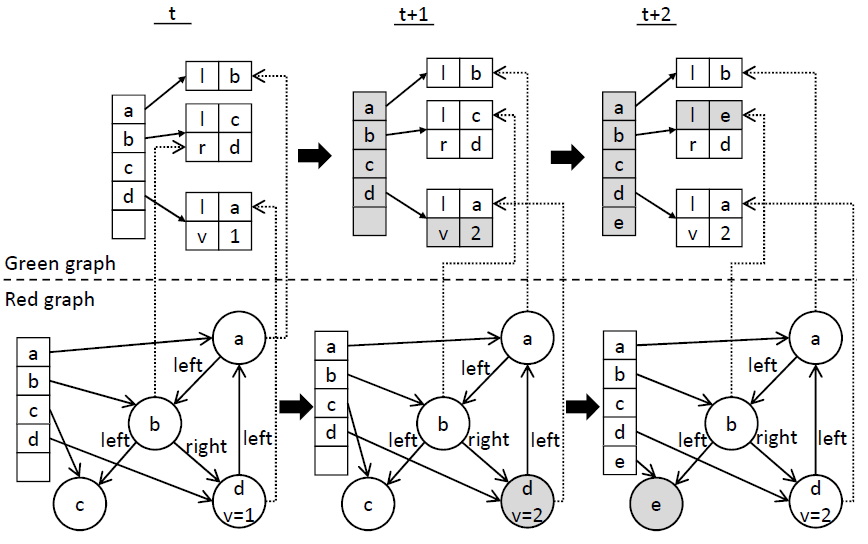
\includegraphics[width=\textwidth]{RedGreenGraph.png}\end{center}

A zöld gráf immutable (perzisztens). A csúcsok egy immutable kulcs-érték tárban vannak eltárolva: a kulcsok a csúcsok azonosítói, az értékek maguk a zöld csúcsok. Egy zöld csúcs ugyancsak egy immutable kulcs-érték tárként van reprezentálva, ahol a kulcsok a csúcs mezőinek nevei, az értékek pedig a mezők értékei. A primitív típusú értékek közvetlenül, a mutató jellegű értékek pedig a célobjektum azonosítójaként vannak tárolva.

A piros gráf egy immutable facade, amely a zöld gráf köré épül on-demand jelleggel: valahányszor egy csomópontra szükség van az azonosítóján keresztüli hivatkozással, a piros gráfban létrejön a meghivatkozott zöld csúcs piros megfelelője. A piros csúcsok az azonosítók alapján cache-elve vannak, így egy későbbi hivatkozás esetén újrahasznosíthatók. Amikor egy mutató jellegű hivatkozást kérdezünk le egy piros csúcsból, a neki megfelelő zöld csúcsban tárolt azonosító feloldódik, és a hivatkozott zöld csúcs piros megfelelőjét kapjuk vissza, amely ugyancsak cache-elődik. A piros csúcsokbók lekérdezett mezők is cache-elve vannak, így csak egyszer kell őket kiértékelni. Kívülről a piros gráf éppen úgy néz ki, mint egy módosítható típusos objektumgráf csak olvasható változata.

\section{Szöveges konkrét szintaxis a Meta-Model nyelvhez}

A Meta-Model nyelv egy tömör és emberek által is könnyen olvasható leírási módot biztosít metamodellek definiálására. A MetaDslx keretrendszer C\# osztályokat generál ebből a leírásból. Ezek a C\# osztályok biztosítják a metamodell implementációjának alapját, amely szálbiztos immutable osztályokból és ugyancsak szálbiztos builder osztályokból áll.

A következő szakaszok részletes leírást adnak a Meta-Model nyelv elemeiről:

\begin{itemize}
	\item Áttekintés: egy magasszintű áttekintést ad a Meta-Model nyelv lehetőségeiről
	\item Tulajdonságok: a tulajdonságok definiálásának és a közöttük lévő kapcsolatokról ad leírást
	\item Típusnélküli elérés: leírja, hogy a modell objektumai miként érhetők el általánosan, típusnélküli módon
	\item Meta-Meta-Model: ez a metamodellje magának a Meta-Model nyelvnek a saját szintaxisában (a Meta-Model nyelv saját magát is képes leírni)
\end{itemize}

\subsection{Áttekintés}

Ez egy magasszintű áttekintés a Meta-Model nyelv képességeiről.

\subsubsection{A Meta-Model kód}

Egy DSL metamodelljét egy '.mm' kiterjesztésű fájlban kell leírni. A metamodell leírása névterekből, osztályokból és asszociációkból áll:

\begin{mmcode}
namespace Sample.Namespace
{
	metamodel MyLanguage(Uri="http://example.org/mylang/1.0"); 
	
	abstract class Person
	{
		string Name;
	}
	
	class Husband : Person
	{
		Wife Wife;
	}
	
	class Wife : Person
	{
		Husband Husband;
	}
	
	association Husband.Wife with Wife.Husband;
}

\end{mmcode}

A névterek ugyanazzal a szintaxissal és jelentéssel bírnak, mint a C\# nyelvben. Az osztályoknak lehetnek tulajdonságaik és műveleteik, támogatják a többszörös öröklődést is. A tulajdonságok lehetnek egyértékűek vagy pedig gyűjtemények. Az asszociációk tulajdonságokat kötnek össze úgy, hogy ha az asszociáció egyik végén beállítjuk a tulajdonság értékét, akkor a másik végének értéke automatikusan beáll a megfelelő értékre.

\subsubsection{A generált C\# implementáció}

A fenti Meta-Model kódból az alábbi publikus C\# API keletkezik:

\begin{csharpcode}
namespace Sample.Namespace
{
	public interface Person
	{
		string Name { get; }
	}
	
	public interface PersonBuilder
	{
		string Name { get; set; }
		Func<string> NameLazy { get; set; }
	}
	
	
	public interface Husband : Person
	{
		Wife Wife { get; }
		string GetWifeName();
		
		HusbandBuilder ToMutable();
		HusbandBuilder ToMutable(MetaDslx.Modeling.MutableModel model);
	}
	
	public interface HusbandBuilder : PersonBuilder
	{
		WifeBuilder Wife { get; set; }
		Func<WifeBuilder> WifeLazy { get; set; }
		
		Husband ToImmutable();
		Husband ToImmutable(MetaDslx.Modeling.ImmutableModel model);
	}
	
	
	public interface Wife : Person
	{
		Husband Husband { get; }
		
		WifeBuilder ToMutable();
		WifeBuilder ToMutable(MetaDslx.Modeling.MutableModel model);
	}
	
	public interface WifeBuilder : PersonBuilder
	{
		HusbandBuilder Husband { get; set; }
		Func<HusbandBuilder> HusbandLazy { get; set; }
		
		Wife ToImmutable();
		Wife ToImmutable(MetaDslx.Modeling.ImmutableModel model);
	}
	
	
	public class MyLanguageFactory
	{
		public MyLanguageFactory(MetaDslx.Modeling.MutableModel model) {/*...*/}
		public HusbandBuilder Husband() { /* ... */ }
		public WifeBuilder Wife() { /* ... */ }
	}
}
\end{csharpcode}


\subsubsection{Egy modell felépítése C\# kódból}

A fenti generált C\# API alapján a következő módon lehet egy példányt (modellt) készíteni a DSL metamodelljéből:

\begin{csharpcode}
MetaDslx.Modeling.MutableModel model = new MetaDslx.Modeling.MutableModel();
MyLanguageFactory factory = new MyLanguageFactory(model);
HusbandBuilder husband = factory.Husband();
husband.Name = "Joe";
WifeBuilder wife = factory.Wife();
wife.NameLazy = () => "Jane";
husband.Wife = wife;
// *** Note that you do not need this:
// wife.Husband = husband; 
// *** since the Wife.Husband and Husband.Wife properties are in an association
\end{csharpcode}

Először egy \ff{MutableModel} objektumot kell készíteni, majd pedig átadni ezt egy olyan factory-nak, amely képes a definiált DSL objektumait létrehozni (\ff{MyLanguageFactory}). Maga a generált builder API a szokásos C\# mutable szintaxist követi, így a modell kényelmesebben megépíthető, mint egy fluent API segítségével.

A builder objektumok mögött is immutable adatszerkezetek vannak, amely minden egyes builder-en keresztül történő módosítás hatására frissülnek.

\subsubsection{Mutable és immutable modellek közötti konverzió}

Egy mutable modell átalakítható immutable modellé a következő módon:

\begin{csharpcode}
MetaDslx.Modeling.ImmutableModel imodel = model.ToImmutable();
\end{csharpcode}

Egy immutable modell átalakítható mutable modellé a következő módon:

\begin{csharpcode}
MetaDslx.Modeling.MutableModel model2 = imodel.ToMutable();
\end{csharpcode}

Alapértelmezetten ez a megoldás az eredeti mutable modellt adja vissza, amelyből az immutable modell készült, még akkor is, ha az a mutable modell időközben megváltozott (gyenge perzisztencia).

Ez a viselkedés azonban felülírható, és egy új verzióág indítható (erős perzisztencia), ha a \ff{ToMutable()} függvénynek egy \ff{true} paramétert adunk át:

\begin{csharpcode}
// This is the default behavior: returns the original mutable model even if it has changed since the immutable model was created
MetaDslx.Modeling.MutableModel model3 = imodel.ToMutable(false); 

// This creates a new mutable model from the current immutable model:
MetaDslx.Modeling.MutableModel model4 = imodel.ToMutable(createNew: true);
\end{csharpcode}

\subsubsection{Mutable objektumok immutable objektummá konvertálása}

A mutable objektumok immutable objektummá konvertálhatók a következő módon:

\begin{csharpcode}
Husband ihusband = husband.ToImmutable();
Wife iwife = wife.ToImmutable();
// *** The following expressions are true:
// ihusband.Wife == iwife
// iwife.Husband == ihusband
\end{csharpcode}

A fenti megoldás azonban csak akkor korrekt, ha a mutable objektumokat tartamlazó mutable modell nem változik időközben. Ha a modell változhat, akkor a következő kódot érdemes használni:

\begin{csharpcode}
// *** We have created the immutable model 'imodel' above
Husband ihusband2 = husband.ToImmutable(imodel);
Wife iwife2 = wife.ToImmutable(imodel);
// *** The following expressions are true:
// ihusband2.Wife == iwife2
// iwife2.Husband == ihusband2
\end{csharpcode}

Az \ff{imodel} paraméter átadva a \ff{ToImmutable()} függvénynek garantálja, hogy a visszatérési értékként kapott objektumok az \ff{imodel} immutable modellből származnak, és mindig konzisztensek.

\subsubsection{Immutable objektumok mutable objektummá konvertálása}

Az immutable objektumok mutable objektummá konvertálhatók a következő módon:

\begin{csharpcode}
HusbandBuilder husband2 = ihusband.ToMutable();
WifeBuilder wife2 = iwife.ToMutable();
// *** The following expressions are true:
// husband2.Wife == wife2
// wife2.Husband == husband2
\end{csharpcode}

A fenti kódban a mutable objektumok ugyanazok, mint azok az objektumok, amelyekből az immutable modell eredetileg keletkezett, még akkor is, ha az a mutable modell időközben megváltozott (gyenge perzisztencia).

Ezért van az, hogy az immutable modell \ff{ToMutable()} függvénye mindig az eredeti mutable modellt adja vissza. Ez garantálja, hogy mindig csak egy mutable verzió van egy modellből, de annak akár több immutable pillanatképe is lehet.

A fenti viselkedés ugyanakkor felülbírálható, ha a mutable modellt átadjuk paraméterként a \ff{ToMutable()} függvénynek:

\begin{csharpcode}
HusbandBuilder husband3 = ihusband.ToMutable(model4);
WifeBuilder wife3 = iwife.ToMutable(model4);
// *** The following expressions are true:
// husband3.Wife == wife3
// wife3.Husband == husband3
\end{csharpcode}

Ilyenkor a \ff{ToMutable()} függvény által visszaadott objektumok a \ff{model5} mutable modellből jönnek.

\subsubsection{Notes on mutable and immutable conversions}

Mind a mutable és az immutable modellek ugyanazt az immutable adatszerkezetet használják a háttérben. Így ugyan a builder objektumok műveletei költségesek lehetnek, egyetlen művelet sem igényel lock-olást, mégis mindegyik szálbiztos. Ezen kívül a mutable és az immutable modellek közötti konverzió mindkét irányban konstans idejű.

Maga a mutable modell tartalmazhat lusta kiértékelésű tulajdonságokat. Ezeket a \ff{ToImmutable()} konverzió alapértelmezett működése során ki fogja értékelni, így ilyenkor a konverziós művelet nem feltétlenül konstans idejű, de ha nincsenek lusta kiértékelésű tulajdonságok, a konstans konverziós idő garantált.

Ha szeretnénk elkerülni a lusta tulajdonságok kiértékelését, akkor egy \ff{false} paraméterrel kell meghívnunk a \ff{ToImmutable()} függvényt:
\begin{csharpcode}
MetaDslx.Modeling.ImmutableModel imodel2 = model.ToImmutable(evaluateLazyValues: false);
\end{csharpcode}

\section{Tulajdonságok}

Ez a szakasz azt írja le, hogyan lehet tulajdonságokat definiálni a Meta-Model nyelvben. Két tulajdonság lehet egymással asszociációban, amely azt jelenti, hogy ha az egyik oldal értékét beállítjuk, akkor a másik oldal értéke automatikusan beáll a megfelelő értékre. A tulajdonságok lehetnek egyszerű értékkel rendelkezők, de lehetnek valamilyen gyűjtemények is. Egy tulajdonság felüldefiniálhat egy másik tulajdonságot, például egy speciálisabb típussal. Egy tulajdonság lehet részhalmaza egy másik tulajdonságnak, amely azt jelenti, hogy ha a részhalmazhoz hozzáadunk egy értéket, akkor az érték a szuperhalmazban is automatikusan megjelenik.

\subsubsection{Asszociációk}

Tekintsük az alábbi Meta-Model leírást:

\begin{mmcode}
namespace Sample.Namespace
{
	metamodel MyLanguage(Uri="http://example.org/mylang/1.0"); 
	
	abstract class Person
	{
		string Name;
	}
	
	class Husband : Person
	{
		Wife Wife;
	}
	
	class Wife : Person
	{
		Husband Husband;
	}
	
	association Husband.Wife with Wife.Husband;
}
\end{mmcode}

Az asszociációk két tulajdonságot kötnek össze. Ha az egyik értékét beállítjuk valamire, a másik értéke automatikusan beáll a megfelelő értékre.

\subsubsection{Gyűjtemények}

A tulajdonságok gyűjtemények is lehetnek:

\begin{mmcode}
class Person
{
	list<Pet> Pets;
}

class Pet
{
	Person Owner;
}

association Person.Pets with Pet.Owner;

class User
{
	set<Role> Roles;
}

class Role
{
	set<User> Users;
}

association User.Roles with Role.Users;
\end{mmcode}

Az asszociációk gyűjtemény jellegű tulajdonságokon is működnek.

A Meta-Model nyelv az alábbi gyűjteményeket támogatja:
\begin{itemize}
	\item \ff{set}: halmaz, az elemek egyediek, a sorrend nem feltétlenül garantált
	\item \ff{list}: lista, az elemek egyediek, az elemek egymáshoz képesti sorrendjét megtartja, indexelhető
	\item \ff{multi\_set}: az elemek nem egyediek, a sorrend nem feltétlenül garantált
	\item \ff{multi\_list}: az elemek nem egyediek, az elemek egymáshoz képesti sorrendjét megtartja, indexelhető
\end{itemize}


\subsubsection{Tulajdonságok felüldefiniálása}

Egy tulajdonság felüldefiniálhat egy másikat ugyanabból az osztályból vagy valamely ősosztályból:

\begin{mmcode}
class Person
{
	list<Pet> Pets;
}

class Pet
{
	Person Owner;
}

association Person.Pets with Pet.Owner;

class Student : Person
{
	list<Dog> Dogs redefines Person.Pets;
}

class Dog : Pet
{
	Student Friend redefines Pet.Owner;
}

association Student.Dogs with Dog.Friend;
\end{mmcode}

A tulajdonságok felüldefiniálását általában a tulajdonság típusának pontosítására használjuk. Az egymást felüldefiniáló tulajdonságok pontosan ugyanazokat az értékeket tárolják, de mindig a legerősebb kényszereknek megfelelően. Ha egy olyan tulajdonságon keresztül adunk értéket egy ilyen egymást felüldefiniáló tulajdonsághalmaznak, amely a kényszert statikusan nem támogatja, akkor kivétel fog keletkezni.

\subsubsection{Részhalmaz tulajdonságok}

\begin{mmcode}
class Person
{
	list<Pet> Pets;
}

class Pet
{
	Person Owner;
}

association Person.Pets with Pet.Owner;

class Student : Person
{
	list<Dog> Dogs subsets Person.Pets;
}

class Dog : Pet
{
	Student Friend redefines Pet.Owner;
}

association Student.Dogs with Dog.Friend;
\end{mmcode}

Egy tulajdonság lehet részhalmaza egy másik tulajdonságnak. Mindkét tulajdonságnak \ff{set} vagy \ff{list} vagy egyedi értéknek kell lennie. Ha egy elemet belerakunk a részhalmazba, akkor annak a szuperhalmazba automatikusan be kell kerülnie. Ha egy elemet törlünk egy szuperhalmazból, annak minden részhalmazból automatikusan törlődnie kell.

\subsection{Típusnélküli elérés}

A Meta-Model nyelv objektumai egy reflection jellegű típusnélküli API segítségével is használhatók.

\subsubsection{A Meta-Model kód}

Vegyük a következő példát:

\begin{mmcode}
namespace Sample.Namespace
{
	metamodel MyLanguage(Uri="http://example.org/mylang/1.0"); 
	
	abstract class Person
	{
		string Name;
	}
	
	class Husband : Person
	{
		Wife Wife;
	}
	
	class Wife : Person
	{
		Husband Husband;
	}
	
	association Husband.Wife with Wife.Husband;
}
\end{mmcode}

\subsubsection{A generált C\# típusnélküli implementáció}

Az áttekintésben bemutatott típusos C\# API mellett az alábbi elemek is el kell, hogy készüljenek:

\begin{mmcode}
namespace Sample.Namespace
{
	public class MyLanguageInstance
	{
		public static readonly MetaDslx.Modeling.Meta-Model Meta-Model;
		public static readonly MetaDslx.Modeling.ImmutableModel Model;
		
		public static readonly MetaDslx.Modeling.MetaClass Husband;
		public static readonly MetaDslx.Modeling.MetaClass Wife;
		public static readonly MetaDslx.Modeling.MetaProperty Person_Name;
		public static readonly MetaDslx.Modeling.MetaProperty Husband_Wife;
		public static readonly MetaDslx.Modeling.MetaProperty Wife_Husband;
	}
	
	public static class MyLanguageDescriptor
	{
		public const string Uri = "http://example.org/mylang/1.0";
		public static class Person
		{
			public static readonly MetaDslx.Modeling.ModelProperty NameProperty;
		}
		public static class Husband
		{
			public static readonly MetaDslx.Modeling.ModelProperty WifeProperty;
		}
		public static class Wife
		{
			public static readonly MetaDslx.Modeling.ModelProperty HusbandProperty;
		}
	}
}
\end{mmcode}

Itt a \ff{MyLanguageInstance} reprezentálja a saját metamodellünket. Ezt lehet meghivatkozni más DSL-ekből, ha szeretnénk a DSL-eket összekötni egymással. A \ff{MyLanguageInstance} arra is alkalmas, hogy futásidőben típusinformációt nyerjünk ki az egyes objektumok metaosztályairól.

A \ff{MyLanguageDescriptor} tartalmazza a metamodellünk URI-jét, amelyet tipikusan XML-sorosításnál lehet hasznosítani, valamint tartalmazza a metaosztályok tulajdonságainak leíróit. Ezekkel a leírókkal lehet típusos elérés nélkül is hozzáférni az objektumok tulajdonságaihoz.

\subsubsection{A típusnélküli factory}

A típusos \ff{MyLanguageFactory} mellett egy itt látható típusnélküli factory is rendelkezésre áll:

\begin{csharpcode}
public class ModelFactory
{
	public IMeta-Model MMeta-Model { get; }
	public MutableModel MModel { get; }
	public MutableSymbol Create(Type type);
	public MutableSymbol Create(string type);
}
\end{csharpcode}

Az \ff{MModel} tulajdonságon keresztül érhető el az a modell, amelyhez új objektumokat ad hozzá a factory. Az \ff{MMeta-Model} az a metamodell, amelyből a factory a modellobjektumokat legyártja. A fenti factory a típusnélküli \ff{Create()} függvényekkel is használható:
\begin{csharpcode}
MetaDslx.Modeling.MutableModel model = new MetaDslx.Modeling.MutableModel();
ModelFactory factory = new ModelFactory(model);
MutableSymbol husband = factory.Create('Husband');
MutableSymbol wife = factory.Create(typeof(Wife));
\end{csharpcode}

\subsubsection{Típusnélküli objektumok}

A mutable és az immutable objektumok is implementálják az alábbi interfészt:
\begin{csharpcode}
public interface IModelObject : IEquatable<IModelObject>
{
	IMeta-Model MMeta-Model { get; }
	MetaClass MMetaClass { get; }
	ObjectId MId { get; }
	IModel MModel { get; }
	
	string MName { get; }
	IModelObject MType { get; }
	
	IModelObject MParent { get; }
	IReadOnlyList<IModelObject> MChildren { get; }
	
	IReadOnlyList<ModelProperty> MProperties { get; }
	IReadOnlyList<ModelProperty> MAllProperties { get; }
	ModelProperty MGetProperty(string name);
	IReadOnlyList<ModelProperty> MGetProperties(string name);
	
	object MGet(ModelProperty property);
	T MGetValue<T>(ModelProperty property) where T : struct;
	T MGetReference<T>(ModelProperty property) where T : class;
	bool MHasDefaultValue(ModelProperty property);
	bool MHasConcreteValue(ModelProperty property);
	bool MIsSet(ModelProperty property);
}
\end{csharpcode}

\subsubsection{Típusnélküli immutable objektumok}

Minden immutable objektum implementálja az alábbi interfészt:
\begin{csharpcode}
public interface ImmutableObject : IModelObject
{
	new ImmutableModel MModel { get; }
	new ImmutableObject MParent { get; }
	new ImmutableModelList<ImmutableObject> MChildren { get; }
	
	new ImmutableObject MType { get; }
	
	MutableObject ToMutable();
	MutableObject ToMutable(MutableModel mutableModel);
}
\end{csharpcode}

\subsubsection{Típusnélküli mutable objektumok}

Minden mutable objektum implementálja az alábbi interfészt:
\begin{csharpcode}
public interface MutableObject : IModelObject
{
	bool MIsReadOnly { get; }
	new MutableModel MModel { get; }
	new MutableObject MParent { get; }
	new ImmutableModelList<MutableObject> MChildren { get; }
	
	void MAttachProperty(ModelProperty property);
	
	new string MName { get; set; }
	new MutableObject MType { get; set; }
	
	void MSet(ModelProperty property, object value);
	void MSetLazy(ModelProperty property, LazyValue value);
	void MAdd(ModelProperty property, object value);
	void MAddLazy(ModelProperty property, LazyValue value);
	void MAddRange(ModelProperty property, IEnumerable<object> value);
	void MAddRangeLazy(ModelProperty property, IEnumerable<LazyValue> value);
	void MMakeCreated();
	
	void MValidate(DiagnosticBag diagnostics, CancellationToken cancellationToken = default);
	
	ImmutableObject ToImmutable();
	ImmutableObject ToImmutable(ImmutableModel immutableModel);
}
\end{csharpcode}

\subsection{Meta-Meta-Model}

A Meta-Model nyelv saját magát is le tudja írni, vagyis saját magának a metamodellje. Ez a metamodell a következőképpen van definiálva:

\begin{mmcode}
namespace MetaDslx.Languages.Meta.Model
{
	/**
	Represents the Meta-Model.
	*/
	metamodel Meta(Uri="http://metadslx.core/1.0"); 
	
	const MetaPrimitiveType Object = "object";
	const MetaPrimitiveType String = "string";
	const MetaPrimitiveType Int = "int";
	const MetaPrimitiveType Long = "long";
	const MetaPrimitiveType Float = "float";
	const MetaPrimitiveType Double = "double";
	const MetaPrimitiveType Byte = "byte";
	const MetaPrimitiveType Bool = "bool";
	const MetaPrimitiveType Void = "void";
	const MetaPrimitiveType ModelObject = "global::MetaDslx.Modeling.IModelObject";
	
	const MetaAttribute NameAttribute = "NameAttribute";
	const MetaAttribute TypeAttribute = "TypeAttribute";
	const MetaAttribute ScopeAttribute = "ScopeAttribute";
	const MetaAttribute BaseScopeAttribute = "BaseScopeAttribute";
	const MetaAttribute LocalScopeAttribute = "LocalScopeAttribute";
	
	/**
	Represents an element.
	*/
	abstract class MetaElement
	{
		// List of attributes
		list<MetaAttribute> Attributes; 
	}
	
	abstract class MetaDocumentedElement : MetaElement
	{
		string Documentation;
	}
	
	abstract class MetaNamedElement : MetaDocumentedElement
	{
		[Name]
		string Name;
	}
	
	abstract class MetaTypedElement : MetaElement
	{
		[Type]
		MetaType Type;
	}
	
	[Type]
	abstract class MetaType
	{
		bool ConformsTo(MetaType type);
	}
	
	class MetaNamedType : MetaType, MetaDeclaration
	{
	}
	
	class MetaAttribute : MetaNamedElement
	{
	}
	
	abstract class MetaDeclaration : MetaNamedElement
	{
		MetaNamespace Namespace;
		derived Meta-Model Meta-Model;
		derived string FullName;
	}
	
	[Scope]
	class MetaNamespace : MetaDeclaration
	{
		containment Meta-Model DefinedMeta-Model;
		containment list<MetaDeclaration> Declarations;
	}
	
	association MetaNamespace.Declarations with MetaDeclaration.Namespace;
	
	class Meta-Model : MetaNamedElement
	{
		string Uri;
		string Prefix;
		MetaNamespace Namespace;
	}
	
	association MetaNamespace.DefinedMeta-Model with Meta-Model.Namespace;
	
	enum MetaCollectionKind
	{
		List,
		Set,
		MultiList,
		MultiSet
	}
	
	class MetaCollectionType : MetaType
	{
		MetaCollectionKind Kind;
		MetaType InnerType;
		bool ConformsTo(MetaType type);
	}
	
	class MetaNullableType : MetaType
	{
		MetaType InnerType;
		bool ConformsTo(MetaType type);
	}
	
	class MetaPrimitiveType : MetaNamedType
	{
		bool ConformsTo(MetaType type);
	}
	
	[Scope]
	class MetaEnum : MetaNamedType
	{
		containment list<MetaEnumLiteral> EnumLiterals;
		containment list<MetaOperation> Operations;
	}
	
	class MetaEnumLiteral : MetaNamedElement, MetaTypedElement
	{
		MetaEnum Enum redefines MetaTypedElement.Type;
	}
	
	association MetaEnumLiteral.Enum with MetaEnum.EnumLiterals;
	
	class MetaConstant : MetaNamedType, MetaTypedElement
	{
		string DotNetName;
		readonly ModelObject Value;
		bool ConformsTo(MetaType type);
	}
	
	[Scope]
	class MetaClass : MetaNamedType
	{
		bool IsAbstract;
		[BaseScope]
		list<MetaClass> SuperClasses;
		containment list<MetaProperty> Properties;
		containment list<MetaOperation> Operations;
		bool ConformsTo(MetaType type);
		list<MetaClass> GetAllSuperClasses(bool includeSelf);
		list<MetaProperty> GetAllSuperProperties(bool includeSelf);
		list<MetaOperation> GetAllSuperOperations(bool includeSelf);
		list<MetaProperty> GetAllProperties();
		list<MetaOperation> GetAllOperations();
		list<MetaProperty> GetAllFinalProperties();
		list<MetaOperation> GetAllFinalOperations();
	}
	
	[LocalScope]
	class MetaOperation : MetaNamedElement
	{
		MetaClass Class;
		MetaEnum Enum;
		bool IsBuilder;
		bool IsReadonly;
		containment list<MetaParameter> Parameters;
		MetaType ReturnType;
		bool ConformsTo(MetaOperation operation);
	}
	
	association MetaOperation.Class with MetaClass.Operations;
	association MetaOperation.Enum with MetaEnum.Operations;
	
	class MetaParameter : MetaNamedElement, MetaTypedElement
	{
		MetaOperation Operation;
	}
	
	association MetaOperation.Parameters with MetaParameter.Operation;
	
	enum MetaPropertyKind
	{
		Normal,
		Readonly,
		Lazy,
		Derived,
		DerivedUnion
	}
	
	class MetaProperty : MetaNamedElement, MetaTypedElement
	{
		MetaPropertyKind Kind;
		MetaClass Class;
		string DefaultValue;
		bool IsContainment;
		list<MetaProperty> OppositeProperties;
		list<MetaProperty> SubsettedProperties;
		list<MetaProperty> SubsettingProperties;
		list<MetaProperty> RedefinedProperties;
		list<MetaProperty> RedefiningProperties;
		bool ConformsTo(MetaProperty property);
	}
	
	association MetaProperty.Class with MetaClass.Properties;
	association MetaProperty.OppositeProperties with MetaProperty.OppositeProperties;
	association MetaProperty.SubsettedProperties with MetaProperty.SubsettingProperties;
	association MetaProperty.RedefinedProperties with MetaProperty.RedefiningProperties;
}
\end{mmcode}

\chapter{Meta-Generator nyelv}

A Meta-Generator nyelv egy felhasználóbarát sablon alapú kódgenerátor nyelv. Egy ilyen Meta-Generator leírást a MetaDslx keretrendszer C\# kóddá transzformál, amely ténylegesen végrehajtható. A generátorban be lehet járni tetszőleges C\# (vagy .NET) objektumgráfot, így a Meta-Model nyelven leírt modelleket is.

A Meta-Generator nyelv fő előnye más generátor nyelvekhez képest, hogy sokkal felhasználóbarátabb és a generált kód formázása is könnyen kontrollálható.

A Meta-Generator leírás csak transzformálódik C\#-ra, nem történik tényleges fordítás. Ennek köszönhetően az esetleges hibák a C\# kódban jelennek meg, de a C\# kódban lévő sorok végén kommentbe bekerül, hogy az adott rész az eredeti Meta-Generator kódban hol szerepel. Így könnyebb megtalálni, hogy mi okozhatja a hibát, és könnyebb azt kijavítani az eredeti kódban.

A következő szakaszok a Meta-Generator nyelv egyes elemeit specifikálják.

\section{Sablonok}

A Meta-Generator nyelv legfontosabb eleme a sablon. A sablonok definiálják, hogy milyen kimenetet kell generálni. Egy sablon egy olyan C\# függvénnyé alakul át, amely egy egyszerű string értékkel tér vissza. Ez a string fáljba is írható, vagy akár egy másik sablonba beágyazható.

Az alábbi példa egy egyszerű Hello World sablonra mutat példát (HelloGenerator.mgen):

\begin{mgencode}
namespace MGenTutorial;
generator HelloGenerator for object;

template SayHello(string name)
Hello, [name]!
end template
\end{mgencode}

A sablonoknak lehetnek paramétereik. A paraméterezés szintaxisa ugyanolyan, mint a C\# nyelvben.

A sablon tartalma a sablon kimenetének részét képezi. A szögletes zárójelek között megadott kód vezérlésre használható. Minden, ami a szögletes zárójeleken kívül van, közvetlenül a kimenetre megy.

Így lehet a generátort C\#-ból meghívni:

\begin{csharpcode}
namespace MGenTutorial
{
	class Program
	{
		static void Main(string[] args)
		{
			HelloGenerator generator = new HelloGenerator();
			string output = generator.SayHello("World");
			Console.WriteLine(output);
		}
	}
}
\end{csharpcode}

A program az alábbi kimenetet fogja adni:

\begin{textcode}
Hello, World!
\end{textcode}

A fenti kódnak azért kell működnie, mert a HelloGenerator.mgen fájlból egy HelloGenerator.cs C\# kód keletkezik, valamilyen az alábbihoz hasonló tartalommal:

\begin{csharpcode}
namespace MGenTutorial
{
	public class HelloGenerator
	{
		public HelloGenerator()
		{
		}
		
		public string SayHello(string name)
		{
			// C# code translated from the SayHello template
		}
	}
}
\end{csharpcode}

\section{Függvények}

A Meta-Generator nyelvben függvények is definiálhatók. A függvények és a sablonok egymást is meghívhatják.

Egy függvény szignatúrája ugyanolyan, mint a C\# nyelven, de azt meg kell előznie a \ff{function} kulcsszónak. A függvény végét az \ff{end function} sor zárja. A függvényen belül a vezérlőszerkezetek a Meta-Generator nyelv vezérlőszerkezeteit kell, hogy kövessék, de a kifejezések a C\# nyelv szintaxisát követik.

Például:

\begin{mgencode}
function void Main()
  Console.WriteLine(MainTemplate());
end function

template T1(string a)
template [a]
end template

function string F1(string a)
  return "function "+a;
end function

template MainTemplate()
  This code shows how to call functions and 
  templates from each other:
    [F1("F1")]
    [T1("T1")]
end template
\end{mgencode}

A generátor \ff{Main()} függvényét a következőképpen hívhatjuk meg C\#-ból:

\begin{csharpcode}
namespace MGenTutorial
{
	class Program
	{
		static void Main(string[] args)
		{
			HelloGenerator generator = new HelloGenerator();
			generator.Main();
		}
	}
}
\end{csharpcode}

A fenti kódnak az alábbi eredményt kell kinyomtatnia:

\begin{textcode}
  This code shows how to call functions and
  templates from each other:
function F1
template T1
\end{textcode}

\section{Formázás}

A Meta-Generator nyelv legfőbb erőssége, hogy a kimenet formázása nagyon jól vezérelhető.

Az alábbi formázási szabályok érvényesek a sablonokra:
\begin{itemize}
	\item Az üres sorok automatikusan törlődnek.
	\item Egy üres sor akkor marad csak meg a kimeneten, ha azt explicit a kalap jellel (\ff{\^}) jelöltük.
	\item Ha nem szeretnénk automatikusan új sort kezdeni egy sor végén, akkor a visszaper jelet (\ff{$\backslash$}) kell elhelyezni a sor végén.
\end{itemize}

A következő sablon ezeket a szabályokat demonstrálja:

\begin{mgencode}
template EmptyLines()
  Apple
^
  Pear

  Green
  [Empty1()]
  Blue

  Black
  [Empty2()]
  White

  First, \
Second, \
Third
end template

template Empty1()

end template

template Empty2()
^
end template
\end{mgencode}

The EmptyLines() template outputs:

\begin{textcode}
  Apple

  Pear
  Green
  Blue
  Black

  White
  First, Second, Third
\end{textcode}

Ha egy sablonon belül meghívunk egy másik sablont vagy függvényt, amely több soros szöveggel tér vissza, akkor azok a sorok mind ugyanazzal a bekezdéssel kerülnek kiírásra. Ez a bekezdés az a szóköz és tab sorozat, amely a sablon illetve függvény meghívása sorának elején található. Például:

\begin{mgencode}
template Indent1()
  Indent1 - line 1
  [Indent2()]
  Indent1 - line 2
end template

template Indent2()
  Indent2 - line 1
  [Indent3()]
  Indent2 - line 2
end template

template Indent3()
  Indent3 - line 1
  Indent3 - line 2
end template
\end{mgencode}

Az \ff{Indent1()} sablon kimenete:

\begin{textcode}
  Indent1 - line 1
    Indent2 - line 1
      Indent3 - line 1
      Indent3 - line 2
    Indent2 - line 2
  Indent1 - line 2
\end{textcode}

A bekezdések megtartása nagyon fontos a szép formázott kód előállításához.

\section{Utasítások}

A kifejezések és változódeklarációk ugyanazt a szintaxist követik, mint a C\# nyelvben. Azonban az olvashatóság megkönnyítése miatt a vezérlőszerkezetek eltérnek a C\# szintaxisától.

A Meta-Generator nyelv az alábbi vezérlési szerkezeteket támogatja:
\begin{itemize}
	\item return
	\item if
	\item switch
	\item typed switch
	\item while
	\item repeat
	\item loop
\end{itemize}

\bb{return utasítás}

A visszatérési (\ff{return}) utasítás szintaxisa megegyezik a C\# szintaxisával, és csak függvényen belül használható. A sablonokban nem szerepelhet visszatérési utasítás.

Az alábbi példa azt mutatja meg, hogyan lehet változókat deklarálni, és hogyan lehet a \ff{return} utasítást használni:

\begin{mgencode}
template SumT1(int a, int b)
  [int sum = a+b]
  [int prod]
  [prod = a*b]
  The sum of [a]+[b] is [sum]
  The product of [a]*[b] is [prod]
end template

function int SumF1(int a, int b)
  int sum = a+b;
  int prod;
  prod = a*b;
  return sum;
end function
\end{mgencode}

Ha a \ff{SumT1} sablont az \ff{a=3} és \ff{b=5} paraméterekkel hívjuk, az alábbi eredményt kell, hogy kapjuk:

\begin{textcode}
  The sum of 3+5 is 8
  The product of 3*5 is 15
\end{textcode}

Figyeljük meg, hogy a váltózó deklarációk és értékadások nem jelennek meg a sablon kimenetében. Így a sablonban nyugodtan elhelyezhetünk segédváltozókat anélkül, hogy az értékük megjelenne a kimeneten.

\bb{if utasítás}

Az \ff{if} utasítás feltételes elágazást jelent. Az \ff{if} utasítás az alábbi szintaxist követi:

\begin{mgencode}
if (condition1)
// ...
else if (condition2)
// ...
else if (condition3)
// ...
else
// ...
end if
\end{mgencode}

Az \ff{else if} és az \ff{else} ágak opciónálisak, de az \ff{if} utasítást végül \ff{end if} sorral kell zárni. A C\# nyelv kapcsoszárójelei helyett a fenti szintaxist kell használni, mivel ezek a sablonokban is jobb olvashatóságot eredményeznek.

Az alábbi példák az \ff{if} vezérlésre mutatnak példát sablonokban és függvényekben:

\begin{mgencode}
template IfT1(int a, string msg)
  [if (a > 0)]
positive
  [else if (a < 0)]
negative
  [else]
[msg]
  [end if]
end template

function string IfF1(int a, string msg)
  if (a > 0)
    return "positive";
  else if (a < 0)
    return "negative";
  else
    return msg;
  end if
end function

template IfT2()
Templates:
  [IfT1(1, "hello")]
  [IfT1(-1, "hello")]
  [IfT1(0, "hello")]
Functions:
  [IfF1(1, "hello")]
  [IfF1(-1, "hello")]
  [IfF1(0, "hello")]
end template
\end{mgencode}

Az \ff{IfT2} sablon kimenete a következő:

\begin{textcode}
Templates:
  positive
  negative
  hello
Functions:
  positive
  negative
  hello
\end{textcode}

\bb{switch utasítás}

A \ff{switch} utasítással egy változó lehetséges értékeit lehet megkülönböztetni egymástól. A szintaxis a következő:

\begin{mgencode}
switch (variable)
case value1:
// ...
case value2, value3:
// ...
default:
// ...
end switch
\end{mgencode}

Az esetek darabszáma tetszőleges, és mind a \ff{case} ágak, mint a \ff{default} ág opcionális. Az egyes ágak nem tudnak továbbfutni egymásra, mert a \ff{switch} valójában \ff{if-else} értékek sorozatává fordul:

\begin{mgencode}
if (variable == value1)
// ...
else if (variable == value2 || variable == value3)
// ...
else
// ...
end if
\end{mgencode}

Az alábbi példák a \ff{switch} vezérlésre mutatnak példát sablonokban és függvényekben:

\begin{mgencode}
template SwitchT1(int a, string msg)
  [switch (a)]
  [case 1:]
one
  [case 2:]
two
  [case 3, 4:]
three or four
  [default:]
[msg]
  [end switch]
end template

function string SwitchF1(int a, string msg)
  switch (a)
  case 1: return "one";
  case 2: return "two";
  case 3, 4: return "three or four";
  default: return msg;
  end switch
end function

template SwitchT2()
Templates:
  [SwitchT1(1, "hello")]
  [SwitchT1(3, "hello")]
  [SwitchT1(0, "hello")]
Functions:
  [SwitchF1(1, "hello")]
  [SwitchF1(4, "hello")]
  [SwitchF1(0, "hello")]
end template
\end{mgencode}

Az \ff{SwitchT2} sablon kimenete a következő:

\begin{textcode}
Templates:
  one
  three or four
  hello
Functions:
  one
  three or four
  hello
\end{textcode}

\bb{Típusos switch utasítás}

Egyes esetekben az érték típusa alapján kell elágaznunk. Ilyenkor lehet hasznos a típusos \ff{switch} utasítás.

Tegyük fel, hogy az alábbi osztályokat definiáltuk C\#-ban:

\begin{csharpcode}
public class Person
{
	public string Name { get; set; }
}

public class Student : Person
{
	public string StudentId { get; set; }
}

public class Baby : Person
{
	public DateTime BirthDate { get; set; }
}
\end{csharpcode}

Ezek a típusok a generátorban is használhatók. Az alábbi példa a típusos \ff{switch} utasításra mutat példát:

\begin{mgencode}
template TypedSwitchT1(Person p)
  [switch (p)]
  [type as Student:]
[p.StudentId]
  [type as Baby:]
[p.BirthDate]
  [default:]
[p.Name]
  [end switch]
end template

function string TypedSwitchF1(Person p)
  switch (p)
  type as Student: return p.StudentId;
  type as Baby: return p.BirthDate.ToString();
  default: return p.Name;
  end switch
end function
\end{mgencode}

Figyeljük meg, hogy habár a bejövő \ff{p} paraméter \ff{Person} típusú, a típusos \ff{switch} megfelelő ágaiban a \ff{p} típusspecifikus elemei is elérhetővé válnak.

Az előzőekben bemutatott értékeket vizsgáló \ff{case} esetek és az itt bemutatott \ff{type as} ágak keverhetők is egymással:

\begin{mgencode}
template TypedSwitchT2(Person p)
  [switch (p)]
  [case null:]
null
  [type as Student:]
[p.StudentId]
  [end switch]
end template

function string TypedSwitchF2(Person p)
  switch (p)
  case null: return "null";
  type as Student: return p.StudentId;
  end switch
return "";
end function
\end{mgencode}

\bb{for utasítás}

A \ff{for} utasítás segítségével lehet egy értéktartományon végiglépkedni.

A \ff{for} utasítás szintaxisa az alábbi:

\begin{mgencode}
for (init declaration; end condition; step expression)
// ...
end for
\end{mgencode}

Az alábbi példák a \ff{for} vezérlésre mutatnak példát sablonokban és függvényekben:

\begin{mgencode}
template ForT1()
  [for (int i = 0; i < 5; ++i)]
[i]
  [end for]
end template

function void ForF1()
  for (int i = 0; i < 5; ++i)
    Console.WriteLine(i);
  end for
end function
\end{mgencode}

\bb{while utasítás}

A \ff{while} utasítás segítségével lehet valamit ismételni, amíg egy adott feltétel igaz értékű.

A \ff{while} utasítás szintaxisa az alábbi:

\begin{mgencode}
while (condition)
// ...
end while
\end{mgencode}

Az alábbi példák a \ff{while} vezérlésre mutatnak példát sablonokban és függvényekben:

\begin{mgencode}
template WhileT1()
  [int n = 0]
  [while (n < 5)]
[n++]
  [end while]
end template

function void WhileF1()
  int n = 0;
  while (n < 5)
    Console.WriteLine(n++);
  end while
end function
\end{mgencode}

\bb{repeat utasítás}

A \ff{repeat} utasítás segítségével lehet valamit ismételni, amíg egy adott feltétel igazzá nem válik. Az utasítás törzse legalább egyszer lefut.

A \ff{repeat} utasítás szintaxisa az alábbi:

\begin{mgencode}
repeat
// ...
until (condition)
\end{mgencode}

Az alábbi példák a \ff{repeat} vezérlésre mutatnak példát sablonokban és függvényekben:

\begin{mgencode}
template RepeatT1()
  [int n = 0]
  [repeat]
[n++]
  [until (n == 5)]
end template

function void RepeatF1()
  int n = 0;
  repeat
    Console.WriteLine(n++);
  until (n == 5)
end function
\end{mgencode}

\bb{loop utasítás}

A \ff{loop} utasítás egy kényelmes módot biztosít objektumgráfok bejárására. Egy \ff{loop} utasítás egymásba ágyazott \ff{foreach} utasításokra fordul le C\#-ban.

A \ff{loop} utasítás szintaxisa a következő:

\begin{mgencode}
loop (start->next1->next2)
// ...
end loop
\end{mgencode}

A \ff{next} elemek száma tetszőleges, lehet nulla vagy több. A \ff{start} és a \ff{next} elemeket láncszemeknek nevezzük, és sorrenben egy loop-láncot alkotnak.

A következő példa a \ff{loop} utasítás használatát mutatja be:

\begin{mgencode}
template LoopT1(IEnumerable<Person> persons)
  [loop (p:persons)]
[p.Name]
  [end loop]
end template

function void LoopF1(IEnumerable<Person> persons)
  loop (p:persons)
    Console.WriteLine(p.Name);
  end loop
end function
\end{mgencode}

A \ff{LoopF1} függvényből az alábbi C\# kód keletkezik:

\begin{csharpcode}
void LoopF1(IEnumerable<Person> persons)
{
	foreach (var p in persons)
	{
		Console.WriteLine(p.Name);
	}
}
\end{csharpcode}

Egy láncszem folytatható az ő saját tulajdonságaival vagy függvényeivel. Például:

\begin{mgencode}
template LoopT2(IEnumerable<Person> persons)
  [loop (p:persons->n:Name)]
[n]
  [end loop]
end template

function void LoopF2(IEnumerable<Person> persons)
  loop (p:persons->n:Name)
    Console.WriteLine(n);
  end loop
end function
\end{mgencode}

A fenti példa ugyancsak a \ff{Person} objektumok neveit írja ki. A láncszemek kettőspont előtti prefixe elhagyható, ha a láncszem neve egy érvényes lokális változó a kontextusban. Ilyenkor a láncszem értékére ezen a néven lehet hivatkozni. Például:

\begin{mgencode}
template LoopT3(IEnumerable<Person> persons)
  [loop (p:persons->Name)]
[Name]
  [end loop]
end template

function void LoopF3(IEnumerable<Person> persons)
  loop (p:persons->Name)
    Console.WriteLine(Name);
  end loop
end function
\end{mgencode}

A \ff{LoopF3} C\# megfelelője a következő:

\begin{csharpcode}
void LoopF3(IEnumerable<Person> persons)
{
	foreach (var p in persons)
	{
		foreach (var Name in new string[] { p.Name })
		{
			Console.WriteLine(Name);
		}
	}
}
\end{csharpcode}

A \ff{typeof} láncszem speciális, ezzel az előző láncszem által reprezentált gyűjtemény megfelelő típusú elemeit lehet leválogatni:

\begin{mgencode}
template LoopT4(IEnumerable<Person> persons)
  [loop (p:persons->typeof(Baby)->bd:BirthDate)]
[bd]
  [end loop]
end template

function void LoopF4(IEnumerable<Person> persons)
  loop (p:persons->typeof(Baby)->bd:BirthDate)
Console.WriteLine(bd);
  end loop
end function
\end{mgencode}

Figyeljük meg, hogy a \ff{typeof} láncszem után már használhatók a típusspecifikus tulajdonságok és függvények is.

A láncszemek a \ff{where} kulcsszó segítségével is szűrhetők:

\begin{mgencode}
template LoopT5(IEnumerable<Person> persons)
  [loop (p:persons->b:typeof(Baby) where b.BirthDate.Year > 2000 && b.Name.StartsWith("A"))]
[b.Name]
  [end loop]
end template

function void LoopF5(IEnumerable<Person> persons)
  loop (p:persons->b:typeof(Baby) where b.BirthDate.Year > 2000 && b.Name.StartsWith("A"))
    Console.WriteLine(b.Name);
  end loop
end function
\end{mgencode}

A \ff{LoopT5} és \ff{LoopF5} is azon 2000 után született gyerekek neveit sorolja fel, akiknek a neve 'A' betűvel kezdődik.

Egy másik hasznos \ff{loop} elem a \ff{separator}. Egy szeparátor akkor lehet hasznos, ha elemek egy listáját kell kiíratni valamilyen speciális szöveggel (tipikusan vesszővel) elválasztva. A szeparátorok mindig string értékűek, és a következőképpen használhatók:

\begin{mgencode}
template LoopT6(IEnumerable<Person> persons)
  [loop (p:persons; separator sep = ", ")]
[p.Name][sep]\
  [end loop]
end template

function void LoopF6(IEnumerable<Person> persons)
  loop (p:persons; separator sep = ", ")
    Console.Write(p.Name);
    Console.Write(sep);
  end loop
end function
\end{mgencode}

A szeparátorok száma mindig eggyel kevesebb, mint a kiírt elemek száma. Az utolsó elemnél a szeparátor üres karakterlánc, minden más elemnél a \ff{loop} fejlécében definiált érték.

Néha arra is szükség lehet, hogy eldöntsük, hogy egy adott \ff{loop} rendelkezik-e egyáltalán eredménnyel. Ennek eldöntésére használható a \ff{hasloop} függvény, amely fejléce pontosan ugyanolyan szintaxisú, mint a \ff{loop} fejléce. A \ff{hasloop} függvény pontosan akkor tér vissza igazzal, ha egy ugyanilyen \ff{loop} törzse legalább egyszer lefutna. Például:

\begin{mgencode}
template LoopT7(IEnumerable<Person> persons)
  [if (hasloop(p:persons where p.Name.StartsWith("A")))]
Persons whose name start with the letter 'A':
    [loop (p:persons; separator sep = ", ")]
[p.Name][sep]\
    [end loop]
  [end if]
end template

function void LoopF7(IEnumerable<Person> persons)
  if (hasloop(p:persons where p.Name.StartsWith("A")))
    Console.WriteLine("Persons whose names start with the letter 'A':");
    loop (p:persons where p.Name.StartsWith("A"); separator sep = ", ")
      Console.Write(p.Name);
      Console.Write(sep);
    end loop
  end if
end function
\end{mgencode}

\section{Konfiguráció}

Egy Meta-Generator fájl az alábbi elemeket tartalmazza az alábbi sorrendben:
\begin{itemize}
	\item namespace deklaráció
	\item generator deklaráció
	\item using deklarációk
	\item properties deklaráció
	\item external függvények
	\item generátor sablonok és függvények
\end{itemize}

\bb{namespace és generator deklaráció}

A \ff{namespace} deklaráció adja meg a C\# névteret, a \ff{generator} deklaráció adja meg a C\# osztály nevét, amely a Meta-Generator kódból jön létre.

A \ff{generator} deklaráció adja meg az objektumgráf gyökerét is, amelyet a generátor be tud járni. A generátoron belül a gyökér neve \ff{Instances}, típusa tetszőleges lehet, de általában valamilyen gyűjtemény szokott lenni. Például:

\begin{mgencode}
namespace MGenTutorial;
generator HelloGenerator for IEnumerable<Person>;

template ListNames()
  [loop(p:Instances; separator sep = ", ")]
[p.Name][sep]\
  [end loop]
end template
\end{mgencode}

Ebből az alábbi C\# kód keletkezik:

\begin{csharpcode}
namespace MGenTutorial //1:1
{
	public class HelloGenerator //2:1
	{
		private IEnumerable<Person> Instances; //2:1
		
		public HelloGenerator() //2:1
		{
		}
		
		public HelloGenerator(IEnumerable<Person> instances) : this() //2:1
		{
			this.Instances = instances;
		}
		
		public string ListNames() //4:1
		{
			// ...
		}
	}
}
\end{csharpcode}

A gyökér objektumot a konstruktorban kell átadni. A generátort így lehet meghívni C\#-ból:

\begin{csharpcode}
namespace MGenTutorial
{
	public class Person
	{
		public string Name { get; set; }
	}
	
	class Program
	{
		static void Main(string[] args)
		{
			List<Person> persons = new List<Person>();
			persons.Add(new Person() { Name = "Alice" });
			persons.Add(new Person() { Name = "Bob" });
			HelloGenerator generator = new HelloGenerator(persons);
			Console.WriteLine(generator.ListNames());
		}
	}
}
\end{csharpcode}

Ez a következő kimenetet adja:

\begin{textcode}
Alice, Bob
\end{textcode}

A generált C\# kódnak kommenteket is tartalmaznia kell, hogy az egyes elemek a Meta-Generator leírás mely sorából és oszlopából származnak. Mivel a Meta-Generator leírás nem fordítással, csak egy transzformációval alakul át C\# kóddá, egyes fordítási hibák csak a C\# kódban derülnek ki. A kommentek segítenek a hiba helyének visszakeresésében a Meta-Generator leírásban.

Ha a generátor egy DSL számára készül, akkor a gyökér típusa általában \ff{IEnumerable<IModel\-Object>}, vagyis a DSL modellobjektumainak listája.

\bb{using deklarációk}

A \ff{using} deklarációk segítségével lehet .NET névtereket importálni a generátorba, illetve más generátorok sablonjait és függvényeit importálni. Így a generátort akár több egységre is szét lehet darabolni.

A \ff{using} deklaráció szintaxisa a következő:

\begin{mgencode}
using MetaDslx.Languages.Meta;
using generator OtherGenerator;
\end{mgencode}

A \ff{using generator} által beimportált generátor sablonjai és függvényei így hívhatók meg:

\begin{mgencode}
template UsingTheOtherGenerator()
[OtherGenerator.SomeTemplate("hello")]
[OtherGenerator.SomeFunction(Instances)]
end template
\end{mgencode}

Az importált generátor nem ismeri az \ff{Instances} tulajdonságát az importáló generátornak, így a megfelelő objektumokat paraméterként kell átadni a megfelelő sablonoknak és függvényeknek.

\bb{properties deklaráció}

Egy generátort általában fel kell konfigurálni valamilyen módon. Erre szolgálnak a generátor tulajdonságai. Ezeket a \ff{properties} deklarációban lehet megadni, és akár hierarchikus csoportosítást is lehet készíteni. A tulajdonságoknak van típusa és alapértelmezett értéke. Például:

\begin{mgencode}
namespace MGenTutorial;
generator HelloGenerator for IEnumerable<Person>;

properties Properties
  bool GenerateXsd = true;
  string DefaultNamespace = "";
  properties XsdOptions
    bool GenerateElements = false;
  end properties
end properties

template GenerateCSharp()
namespace [Properties.DefaultNamespace]
{
}
end template
\end{mgencode}

A fenti módon definiált generátor a hívó C\# kódból az alábbi módon konfigurálható:

\begin{csharpcode}
class Program
{
	static void Main(string[] args)
	{
		HelloGenerator generator = new HelloGenerator();
		generator.Properties.DefaultNamespace = "MGenTutorial";
		generator.Properties.XsdOptions.GenerateElements = true;
		Console.WriteLine(generator.GenerateCSharp());
	}
}
\end{csharpcode}

Fontos, hogy az importált generátorok nem öröklik meg az importáló generátor tulajdonságait, őket külön kell konfigurálni.

\bb{Külső függvények}

Egy generátor definiálhat külső függvényeket. Ezeket a függvényeket C\#-ban kell implementálni, és így egy kényelmesebb szintaxisban írhatók meg. Mindemellett a generátoron belül úgy használhatók, mint a C\# extension függvényei, így a generátor kódja is kényelmesebbé válik. Természetesen ilyen kiterjesztő függvények magában a C\# nyelvben is definiálhatók és a generátorból is meghívhatók.

Egy külső függvényt az \ff{extern function} kulcsszavakkal kell definiálni, és csak a függvény fejlécét kell megadni:

\begin{mgencode}
extern function string ToCamelCase(string identifier)
extern function string ToPascalCase(string identifier)
\end{mgencode}

Ha egy generátor ilyen függvényeket definiál, azokat a transzformált C\# kódban egy \\ \ff{I[GeneratorName]Extensions} fogja tartalmazni. Ezt az interfészt kell a C\# kódban \ff{[GeneratorName]Extensions} néven implementálni, és a generátor ennek az osztálynak a függvényeit fogja hívogatni.

Például ha a generátor a két fenti külső függvényt definiálja, akkor a következő C\# interfész keletkezik belőlük:

\begin{csharpcode}
internal interface IHelloGeneratorExtensions
{
	string ToCamelCase(string identifier); //12:8
	string ToPascalCase(string identifier); //13:8
}
\end{csharpcode}

És ezt kell egy C\# osztálynak (HelloGeneratorExtensions.cs) implementálnia:

\begin{csharpcode}
namespace MGenTutorial
{
	class HelloGeneratorExtensions : IHelloGeneratorExtensions
	{
		public string ToCamelCase(string identifier)
		{
			if (string.IsNullOrEmpty(identifier)) return identifier;
			else return identifier[0].ToString().ToLower() + identifier.Substring(1);
		}
		
		public string ToPascalCase(string identifier)
		{
			if (string.IsNullOrEmpty(identifier)) return identifier;
			else return identifier[0].ToString().ToUpper() + identifier.Substring(1);
		}
	}
}
\end{csharpcode}

Ezután ezek a függvények a generátorban is használhatók akár hagyományos függvényként, akár extension függvényként:

\begin{mgencode}
template ListNamesCamelCase()
  [loop(p:Instances; separator sep = ", ")]
[ToCamelCase(p.Name)][sep]\
  [end loop]
end template

template ListNamesPascalCase()
  [loop(p:Instances; separator sep = ", ")]
[p.Name.ToPascalCase()][sep]\
  [end loop]
end template
\end{mgencode}

\bb{sablonok és függvények}

A generátor többi része tartalmazza a sablonokat és a függvényeket.


\chapter{Annotált ANTLR4 nyelv}

A szintaktikai elemzésre (lexer és parser generálás) vannak már jól bevált megoldások. A lexer és a parser könnyen generálhatók automatizált eszközökkel reguláris kifejezésekből illetve CF nyelvtani leírásból (ld. ANTLR4 később), de szükség esetén mindkettő akár kézzel is megírható. Utóbbi akkor lehet hasznos, ha speciális optimalizációt, különböző cache-elési technikákat és minél finomabb hibakezelést szeretnénk megvalósítani.

Jelenleg azonban nem létezik olyan eszköz, amely a szemantikai elemzést teljes egészében el tudná látni. Vannak ugyan kezdeményezések, amelyek valamilyen limitált támogatást nyújtanak például kereszthivatkozások megvalósítására (pl. XText), de sokszor ennél több szemantikai támogatás is automatizálható lenne.

Az ilyen eszközök hiányának legfőbb oka az lehet, hogy ahány programnyelv, annyiféle szemantikai szabály létezik, így nehéz általános és mindenre kiterjedő szemantikai elemzőt készíteni. Mégis, egyszerű C\#/Java-szerű szintaxissal és hozzájuk hasonló szemantikával rendelkező DSL-ek esetén a szemantikai szabályok elég jól általánosíthatók:
\begin{itemize}
	\item vannak primitív és beépített típusok
	\item vannak névterek
	\item lehet definiálni egyéni típusokat
	\item van öröklődés a típusok között
	\item vannak változók és függvények
	\item vannak utasítások
	\item vannak vezérlési szerkezetek (elágazások, ciklusok)
	\item vannak kifejezések
	\item a kód tipikusan strukturált
\end{itemize}

A fenti szemantikai elemek támogatásával DSL-ek egy nagyon nagy csoportját le lehetne fedni, és így új DSL-ek kifejlesztését fel lehetne gyorsítani.

Természetesen, ha egy adott DSL egyéb extra szemantikai szabályokat is tartalmaz, akkor meg kell adni a lehetőséget, hogy ezeket a szabályokat is be lehessen építeni a fordítóba. Ehhez sok bővítési pontot kell definiálnia a MetaDslx keretrendszernek, hogy akár a szintaktikai elemzésnél, akár a deklarációk kigyűjtésénél és akár a szemantikai elemzésnél is testre lehessen szabni a fordító működését.

A Roslyn fordító a C\# és VB nyelvek esetén már támogatja a fenti szemantikai elemeket, és a Roslyn megfelelő általánosításával a MetaDslx keretrendszer is nagyon erőssé válhatna. Sajnos a Roslyn a C\# és VB nyelvekhez van kötve: a szintaktikai elemző teljesen kézzel van megírva, így azt általánosítani nem lehet, és a szimbólumok nagy része is C\# specifikus. Szerencsére azonban a Roslyn-nak van egy a C\# és a VB nyelvektől független belső magja, amely többé-kevésbé általánosnak tekinthető, de legalábbis belátható mennyiségű munkával általánosítható.

Mivel a Roslyn kézzel írt szintaktikai elemzője nem általánosítható, felmerül az igény, hogy a MetaDslx keretrendszer szintaktikai elemzője az ANTLR4-re épüljön. Az ANTLR4 egy széles körben elterjedt és nagy kifejezőerejű szabályrendszerrel rendelkező lexer és parser generátor, így kiváló jelölt lehet. Az egyetlen megoldandó feladat, hogy az ANTLR4 szintaxisfáját a Roslyn fogalmaira képezzük le. Ehhez be kell vezetni néhány apró korlátozást is az ANTLR4 nyelvtanba, de ezek a korlátozások az ANTLR4 kifejezőerejét nem érintik.

Valahol jelölni kell a szemantikai szabályokat is. Az annotációk a modern programnyelvekben eléggé elterjedtek a metaadatok definiálására, így adja magát a lehetőség, hogy az ANTLR4-ből eddig hiányzó annotációkat szemantikai célokra bevezessük. A szabályokat meg lehetne adni egy ANTLR4-től független külön leíróban is, de egyszerűbb és áttekinthetőbb megoldás az annotációk bevezetése, mert így egy helyen lehet leírni a programkód szintaktikáját és szemantikáját is.

A Roslyn szemantikai elemzőjének működése (Binder API) jelenleg nem publikus, csak az eredményként előálló \f{SemanticModel} segítségével lehet szemantikai kérdéseket feltenni. A Binder API általánosítása és megnyitása elengedhetetlen a bővíthetőség szempontjából.

A Roslyn publikus API-ja nagyon jól dokumentált, sok-sok példa érhető el, amelyek segítségével könnyen megtanulható az API használata. A belső működéshez azonban nincs publikusan elérhető doumentáció. Szerencsére a kód követi a clean-code elveket, így könnyen olvasható, de hatalmas kódbázisról van szó, és a működés pontos megértése nem kis feladat. A működés általánosítása pedig még nehezebb. Így tehát a Roslyn általánosított belső működésének dokumentálása is cél, hiszen ennek köszönhetően lehet majd bővíteni a MetaDslx-ben szereplő szemantikai elemzőt, amennyiben valamilyen extra szemantikai szabályra szükségünk van.


\section{ANTLR4}

A fordítás első fázisa, a szintaktikai elemzés (lexer + parser) automatikusan is generálható, ha megadjuk a megfelelő nyelvtani szabályokat. Számos olyan eszköz létezik, amely alkalmas lexer és parser automatikus előállítására. Az egyik legnépszerűbb ilyen eszköz az ANTLR4 \cite{Antlr4}.

Ez a szakasz az ANTLR4 legfontosabb alapelveit ismerteti \cite{Antlr4Guide} és \cite{Antlr4Doc} alapján. A részletekért célszerű felkeresni ezt a két forrást.

Az ANTLR4 egy sokoldalú parser generátor, amely segítsével strukturált szöveges és bináris fájlokat lehet egyszerűen feldolgozni. A fájl struktúráját egy nyelvtan segítségével kell leírni, amely az ANTLR4 speciális formátumát követi.

Például az alábbi nyelvtan olyan szövegek elemzésére alkalmas, ahol a \f{hello} szó után egy az angol ABC kisbetűiből képzett azonosító szerepel, előttük/közöttük/utánuk pedig tetszőlegesen sok szóköz/tab/újsor fordulhat elő:

\begin{antlr4code}
grammar Hello; // Define a grammar called Hello

main : 'hello' ID ; // match keyword hello followed by an identifier
ID : [a-z]+ ; // match lower-case identifiers
WS : [ \t\r\n]+ -> skip ; // skip spaces, tabs, newlines, \r (Windows)
\end{antlr4code}

A fenti nyelvtani leírásból az ANTLR4 az alábbiakat generálja:
\begin{itemize}
	\item{HelloLexer}: a nyelvtanból készült lexer, amely a 'hello' szót, az 'ID' nevű angol ABC kisbetűiből álló tokent és a 'WS' nevű szóközökből/tabokból/újsorokból álló karakterláncokat képes felismerni
	\item{HelloParser}: a nyelvtanból készült parser, amely a lexer által képzett tokenek alapján a szintaxisfát építi fel
	\item{HelloListener}: a nyelvtanból készült listener, amely a szintaxisfa in-order bejárása során keletkező eseményeket képes lekezelni (pl. megérkeztünk egy adott csúcsba, elhagytunk egy csúcsot, terminálist találtunk, stb.)
	\item{HelloVisitor}: a nyelvtanból készült visitor, amely a szintaxisfa bejárását segíti a Visitor tervezési minta alapján
\end{itemize}

Az ANTLR4-re épülő eszközök tipikusan a generált Listener vagy a Visitor osztályból való leszármazással járják be és értelmezik a parser által készített szintaxisfát.

A fenti nyelvtan elfogadja a \f{hello world} szöveget, és az ANTLR4 által generált parser alábbi szintaxisfát építi belőle:

\begin{center}\includegraphics[trim=70 420 740 50,clip,width=0.2\textwidth,page=6]{Images.pdf}\end{center}

Az ANTLR4 számos előnnyel rendelkezik a többi parser generátor eszközhöz képest. Az ANTLR4 egy helyes bemenetet mindig fel tud dolgozni, bármilyen bonyolult legyen is a nyelvtan. Az ANTLR4 generátora minden CF nyelvtant elfogad, kivéve a közvetett balrekurziót tartalmazó nyelvtanokat (a közvetlen balrekurzió megengedett). Sosem kapunk olyan hibákat, hogy a nyelvtan többértelmű lenne vagy hogy a nyelvtani szabályok ütköznének egymással, mint ahogy az a legtöbb más parser generátor eszköz esetén történik.

Az ANTLR4 által használt algoritmus az adaptív LL(*), azaz ALL(*), amely a nyelvtani elemzést nem statikusan, hanem futásidőben dinamikusan végzi. Ez még azelőtt megtörténik, mielőtt a generált parser lefutna. Mivel az ALL(*) algoritmusnak a teljes bemenetre rálátása van, mindig el tudja dönteni, melyik nyelvtani szabályt kell alkalmazni. Egy statikus elemzőnek minden lehetséges inputra fel kell készülnie, és végtelen előretekintéssel kellene dolgoznia. Az ALL(*) elemzés előnye az is, hogy a nyelvtant nem kell a parser algoritmus igényeihez igazítani, mint a legtöbb más parser generátor eszköz esetén.

Habár közvetett balrekurzió nem megengedett, a közvetlen balrekurziót támogatja az ANTLR4, például:

\begin{antlr4code}
expr : expr '*' expr // match subexpressions joined with '*' operator
     | expr '+' expr // match subexpressions joined with '+' operator
     | INT // matches simple integer atom
;
\end{antlr4code}

Egy ilyen szabály balrekurzív, mert a szabály valamely jobb oldalának első eleme a szabályt magát definiáló nemterminális (\f{expr}). Az ANTLR4 elfogadja a fenti szabályt is, és a szabály jobb oldalai között azok sorrendjében precedencia relációt állít fel. Nincs szükség tehát a nyelvtan struktúrájában jelezni a precedenciát, elegendő a szabályok sorrendjét megfelelően megválasztani. Ezzel nagyban leegyszerűsödik a kifejezések nyelvtani leírása.

Az ANTLR4 további előnye, hogy nagyon gyors. Nagy fájlokat is képes néhány milliszekundum alatt elemezni.

\subsection{Nyelvtan}

ANTLR4 esetén a nyelvtant egy nyelvtanfájlban kell leírni. Ez történhet a lexer és a parser együttes megadásával:

\begin{antlr4code}
grammar Hello; // Define a grammar called Hello

main : 'hello' ID ; // match keyword hello followed by an identifier
ID : [a-z]+ ; // match lower-case identifiers
WS : [ \t\r\n]+ -> skip ; // skip spaces, tabs, newlines, \r (Windows)
\end{antlr4code}

De külön is lehet választani a két fájlt (ez az ajánlott megoldás):

\begin{antlr4code}
lexer grammar HelloLexer; // Define a lexer grammar called HelloLexer

ID : [a-z]+ ; // match lower-case identifiers
WS : [ \t\r\n]+ -> skip ; // skip spaces, tabs, newlines, \r (Windows)
\end{antlr4code}

\begin{antlr4code}
parser grammar HelloParser; // Define a parser grammar called HelloParser

options { tokenVocab = HelloLexer; } // Use tokens defined in HelloLexer

main : 'hello' ID ; // match keyword hello followed by an identifier
\end{antlr4code}

A nyelvtanfájl pontos szerkezete itt van dokumentálva: \cite{Antlr4Grammar}.

\subsection{Lexer}

A lexer feladata a forráskód feldarabolása tokenekre, azaz a legkisebb értelmezhető egységekre. Ilyen tokenek a programnyelvekben a kulcsszavak, azonosítók, kommentek, stb. Egy token mindig legalább két információból áll: a token típusa (fajtája), és a forráskódban lévő szöveg, amelyet a lexer a token létrehozásakor felismert. A lexer kimenete tokenek sorozata.

A lexer nyelvtani leírásában kell definiálni a tokeneket, amelyek nevét nagy kezdőbetűvel kell írni. Lehetőség van token-töredékek (\f{fragment}) megadására is. Ezek a töredékek önállóan nem hoznak létre tokent, de a tényleges tokenek ezekből a töredékekből is összeépíthetők, így a tokeneket defináló szabályok egyszerűbbek lehetnek. Például:

\begin{antlr4code}
fragment HexDigit : [0-9a-fA-F];
HexNumber : '0x' HexDigit+;
\end{antlr4code}

Itt a \f{HexDigit} tokentöredék önmagában sosem alkot tokent, de a segítségével definiált \f{HexNumber} már hozhat létre tokent.

A nyelvünk tartalmazhat olyan tokeneket, amelyek a szintaxisfában nem jelennek meg, a fordítás szempontjából lényegtelenek, mégis a kódban előfordulhatnak. Ilyen tokenek például a szóközök, az új sorok és a kommentek is. A token nyelvtani szabálya után írt \f{skip} utasítás segítségével lehet figyelmen kívül hagyni ezeket a tokeneket, ahogy a fenti \f{Hello} példában is szerepelt. Egy másik lehetőség, hogy egyes tokeneket más-más tokensorozatba, úgynevezett csatornába gyűjtünk. A token nyelvtani szabálya után írt \f{channel} utasítás segítségével megadható, hogy az adott token melyik csatornába kerüljün. A parser csak az alapértelmezett (0-ás sorszámú) csatornát használja, a többi csatornát figyelmen kívül hagyja. Például:

\begin{antlr4code}
lexer grammar HelloLexer;

channels
{
	COMMENT,
	WHITESPACE
}

ID : [a-z]+ ; // match lower-case identifiers

CrLf : '\r'? '\n' -> channel(WHITESPACE);  // Skip new lines, put them into the WHITESPACE channel
Whitespace : [\u0020\u0009\u000B\u000C\u00A0\u001A]+ -> channel(WHITESPACE); // Skip spaces and tabs, put them into the WHITESPACE channel

LineComment : '//' ~ [\r\n]*; // Skip comments, put them into the COMMENT channel
\end{antlr4code}

Előfordulhatnak olyan bonyolultabb nyelvek, ahol a lehetséges felismerhető tokenek valamilyen kontextustól függenek. Például az XML nyelvben a nyitótag-en belül szerepelhetnek attribútumok név-érték párokban, de két tag között vagy zárótag-en belül nem. Ilyenkor hasznos lehet az ANTLR4 lexerek esetén a módok (\f{mode}) használata. Megadhatjuk, hogy melyik módban milyen tokenek jöhetnek, adott token felismerésekor válthatunk lexer módot, és lehetőség van a lexer módok veremként való egymásra pakolására is (\f{pushMode}, \f{popMode}). Példaként itt egy részlet egy XML lexer definíciójából:

\begin{antlr4code}
lexer grammar XMLLexer;

// Default "mode": Everything OUTSIDE of a tag
COMMENT     :   '<!--' .*? '-->' ;
			;
SEA_WS      :   (' '|'\t'|'\r'? '\n')+ ;

OPEN        :   '<'                     -> pushMode(INSIDE) ;
XMLDeclOpen :   '<?xml' S               -> pushMode(INSIDE) ;
SPECIAL_OPEN:   '<?' Name               -> more, pushMode(PROC_INSTR) ;

TEXT        :   ~[<&]+ ;        // match any 16 bit char other than < and &

...

// ----------------- Everything INSIDE of a tag ---------------------
mode INSIDE;

CLOSE       :   '>'                     -> popMode ;
SPECIAL_CLOSE:  '?>'                    -> popMode ; // close <?xml...?>
SLASH_CLOSE :   '/>'                    -> popMode ;
SLASH       :   '/' ;
EQUALS      :   '=' ;
STRING      :   '"' ~[<"]* '"'
			|   '\'' ~[<']* '\''
			;
Name        :   NameStartChar NameChar* ;
WS           :   [ \t\r\n]               -> skip ;

...

// ----------------- Handle <? ... ?> ---------------------
mode PROC_INSTR;

PI          :   '?>'                    -> popMode ; // close <?...?>
IGNORE      :   .                       -> more ;
\end{antlr4code}

A lexer szabályok pontos dokumentációja itt található: \cite{Antlr4Lexer}.

\subsection{Parser}

A parser feladata a tokenek sorozata alapján a forráskódot reprezentáló szintaxisfa felépítése. A fa belső csúcsai a megadott nyelvtani szabályok, levelei a lexer által kiadott tokenek. A parser nyelvtani szabályainak nemterminálisai az angol ABC kisbetűivel kezdődnek, terminálisai az előző szakaszban definiált tokenek, amelyek az angol ABC nagybetűivel kezdődnek.

Egy lehetséges nyelvtani szabály például a következő, amely egy értékadás kifejezést ír le:

\begin{antlr4code}
assign : ID '=' expr ';' ; // match an assignment statement like "sp = 100;"
\end{antlr4code}

Az ANTLR4 parser rekurzív-leszálló (recursive-descent) elemzést végez. Az ilyen elemzés fentről lefelé építi a fát, a következő függvényhez hasonló hívásokon keresztül:

\begin{javacode}
// assign : ID '=' expr ';' ;
void assign() { // method generated from rule assign
	match(ID); // compare ID to current input symbol then consume
	match('=');
	expr(); // match an expression by calling expr()
	match(';');
}
\end{javacode}

A \f{match()} függvényhívások azt vizsgálják, hogy a kívánt token érkezett-e, ezek felelnek meg a fa leveleinek. Az egyéb függvényhívások egy-egy nyelvtani szabálynak felelnek meg, és a fában az eggyel lejjebb lévő nyelvtani szabályokat próbálják illeszteni. Minden egyes ilyen függvényhívás egy új belső csomópont létrehozását jelenti a fában.

A fenti példában az \f{assign()} függvény azt ellenőrzi, hogy a megfelelő tokenek a megfelelő sorrendben érkeztek-e, majd egy kifejezést (\f{expr()}) próbál meg illeszteni. Ebben a példában nincsenek alternatívái a szabály jobb oldalának.

Egy szabálynak lehetnek alternatív jobb oldalai is, például:

\begin{antlr4code}
/** Match any kind of statement starting at the current input position */
stat : assign // First alternative ('|' is alternative separator)
     | ifstat // Second alternative
     | whilestat
     ...
;
\end{antlr4code}

Egy ilyen szabály a következő kódra képződik le a parser-ben:

\begin{javacode}
void stat() {
	switch (current_input_token) {
		case ID : assign(); break;
		case IF : ifstat(); break; // IF is token type for keyword 'if'
		case WHILE : whilestat(); break;
		...
		default : // raise no viable alternative exception
	}
}
\end{javacode}

Itt a \f{stat()} függvénynek egy döntést kell hoznia: meg kell jósolnia, mi lesz a következő szabály. Ehhez a következő tokent kell megvizsgálnia, és azalapján dönti el, melyik alternatívát is kövesse. Ezt hívjuk előretekintésnek, vagyis amikor az elemző megnézi a következő tokent vagy tokeneket anélkül, hogy egy \f{match()} segítségével elfogyasztaná őket. Az elemző az előretekintés alapján dönt arról, hogy milyen műveletet végezzen.

Amíg egy szabály jobb oldalai különböző tokenekkel kezdődnek, az előretekintés egyszerű és gyors. Ha azonban vannak azonos tokennel kezdődő alternatívák, szükség lehet a további tokenek figyelembe vételére is. Ilyenkor az elemzőnek több tokennyire is előre kell néznie, sőt, lehet, hogy a bemenet teljes végéig el kell látnia. Szerencsére ezeket a dolgokat az ANTLR4 elemzője automatikusan elvégzi, nekünk ezzel nem kell foglalkoznunk.

Mindezek ellenére mégis előfordulhatnak olyan esetek, amikor a nyelvtani szabályokból nem egyértelmű, pontosan mit is kellene felismerni. Sőt, vannak olyan programnyelvek, ahol nem is lehet egyértemű nyelvtant írni. Ilyen például a C nyelv, ahol a típuskasztolás és a függvényhívás közötti különbség felderítéséhez nincs elég információ:

\begin{ccode}
int aa(int arg) {
	return arg;
}

int foo(int bb) {
	return (aa)(bb); // this is a function call
}
\end{ccode}

\begin{ccode}
typedef struct aa {
	int cc;
}

int foo(int bb) {
	return (aa)(bb); // this is a type-cast
}
\end{ccode}

Ezekben az esetekben, ha az ANTLR4 több alternatívát is helyesnek lát, az elsőt fogja választani. Azonban lehetőség van arra, hogy egy-egy alternatíva elején vagy közepén kapcsoszárójelek között feltételes kifejezéseket (vágókat) tudjunk kiértékelni, és csak akkor legyen elfogadott az adott alternatíva, ha a feltételes kifejezés igazzal tér vissza. A fenti C problémát úgy lehet feloldani, hogy egy előzetes szintaktikai elemzést végzünk, ahol kigyűjtjük a típusneveket, majd egy második szintaktikai elemzést is futtatunk, ahol már a kigyűjtött típusnevek alapján lehet dönteni, hogy típuskasztolásról vagy függvényhívásról van-e szó:

\begin{antlr4code}
expr : '(' {isTypeName($id.text)}? id ')' expr   #typeCastExpression
     | expr '(' exprList ')'                     #functionCallExpression 
     ...
     ;
\end{antlr4code}

Szerencsére a modernebb programnyelvek már figyelnek arra, hogy ilyen többértelmű helyzetek ne fordulhassanak elő.

A parser szabályok pontos dokumentációja itt található: \cite{Antlr4Parser}.


\section{.NET Compiler Platform ("Roslyn")}\label{RoslynAPI}

Ez a szakasz a Microsoft által fejlesztett .NET Compiler Platform ("Roslyn") \cite{Roslyn} működésének alapelveit mutatja be.

A hagyományos fordítók fekete dobozként működnek. A fordító bemenete a forráskód, kimenete pedig a bináris fájlok (dinamikus könyvtárak, futtatható programok). A fordító belső működése kívülről nem látható, és a rengeteg hasznos szemantikai információ, amit a fordító kinyer a kódból, az elveszik a fordítás végeztével.

A modern fejlesztőkörnyezetek (Integrated Development Environment, IDE) azonban erősen támaszkodnak ezekre a szemantikai információkra, például olyan műveleteknél, mint az IntelliSense, refaktorálás, hivatkozási helyek megkeresése, definíció megkeresése. Sok esetben az IDE fejlesztőknek duplikálniuk kell a fordító által is végzett számításokat, hogy az ilyen fejlesztést segítő műveletek megvalósíthatók legyenek.

Egyszerűbb lenne azonban a valódi fordító által kiszámolt információkat felhasználni, így felmerül az igény a fordító belsejének megnyitására. A .NET Compiler Platform ("Roslyn") a Microsoft nyílt forráskódú megoldása éppen ezt teszi lehetővé C\# és Visual Basic (VB) nyelvek esetén.

Ha a fordító belső API-ja megnyílik, akkor lehetőség van akár futási idejű szkripteket is futtatni az alkalmazásunkból, így még rugalmasabb megoldásokat adhatunk a felhasználók kezébe.


\subsection{A Roslyn fordító API-ja}

A Roslyn API a fordító belső működését publikálja ki, így az a fejlesztők számára is elérhetővé válik.

A fordító belseje az alábbi pipeline szerint működik:

\begin{center}\includegraphics[trim=120 100 160 360,clip,width=\textwidth,page=3]{Images.pdf}\end{center}

A pipeline minden egyes fázisa egy külön komponens. Az első fázisban (parsing fázis) a parser tokenekre bontja a forráskódot, majd a programnyelv nyelvtanának megfelelő szintaxisfát épít fel. A második fázisban (deklarációs fázis) a forráskód és az importált metaadatok (DLL-ek) deklarációiból névvel ellátott szimbólumok keletkeznek. A harmadik fázisban (binding fázis) a kódban lévő azonosítók és az előző fázisban készült szimbólumok megfeleltetésére kerül sor. Végül a negyedik fázisban (emit fázis) a fordító által kiszámított összes információ alapján elkészül a kimeneti kód (DLL).

Az egyes fázisokhoz API felület is tartozik:

\begin{center}\includegraphics[trim=120 100 160 260,clip,width=\textwidth,page=3]{Images.pdf}\end{center}

Minden egyes fázis eredménye egy-egy objektummodell, amelyek API-ján keresztül az adott fázisban kiszámolt információk kinyerhetők. A parsing fázis eredménye egy szintaxisfa, a deklarációs fázis eredménye egy hierarchikus szimbólumtábla, a binding fázis eredménye egy szemantikai modell, az emit fázishoz pedig egy IL kódot készítő API tartozik.

A fordító ezeket a fázisokat (komponenseket) fogja össze, és így tud egy teljes fordítást végrehajtani.

A fordító API-jának elegendő információt kell nyújtania ahhoz, hogy a fejlesztőkörnyezet funkcióit mind rá lehessen építeni:

\begin{center}\includegraphics[trim=120 100 160 90,clip,width=\textwidth,page=3]{Images.pdf}\end{center}

Például a kódformázást a szintaxisfán lehet végrehajtani, az osztályok, függvények és változók közötti navigációt a szimbólumtábla segítségével lehet megvalósítani, a refaktoráláshoz a szemantikai modell szükséges, míg debuggolás közben az "Edit and Continue" művelet a fordító mind a négy fázisát használja. A Visual Studio teljes funkcionalitása a Roslyn API-ra épül, ez biztosítja, hogy az API megfelelően széleskörű támogatást nyújt a legtöbb igény kielégítésére.

\subsection{API rétegek}

A Roslyn API-nak két fő rétege van, a fordító réteg és a munkakörnyezet réteg:

\begin{center}\includegraphics[trim=100 180 150 110,clip,width=\textwidth,page=4]{Images.pdf}\end{center}

A fordító réteg három API-t foglal magába: az előző szakaszban ismertetett fordító API (Compiler API), az erre épülő szkript API (Scripting API) és a diagnosztikai API (Diagnostic API). A munkakörnyezet réteg a munkakörnyezet API-t (Workspace API) tartalmazza.

\subsubsection{Compiler API}

A fordító API tartalmazza azokat a szintaktikai és szemantikai objektummodelleket, amelyek a fordítási pipeline során keletkeznek. Ez a réteg ad hozzáférést a fordító egy konkrét meghívásához, azaz egy fordításhoz is. A fordítás egy nem változtatható (immutable) objektummodell, vagyis egy újabb fordítás során új objektummodellt kell építeni, de egy korábbi fordítás bizonyos részei újrahasznosíthatók. Egy fordítás fogja össze a forrásfájlokat, a fordítási opciókat és a hivatkozott könyvtárakat (assembly-ket) is.

\subsubsection{Scripting API}

A szkript API segítségével C\# és VB kódrészletek fordíthatók és futtathatók futásidőben, sőt, a szkriptek egymásra is épülhetnek felhasználva a korábbi számítások során keletkező eredményeket.

\subsubsection{Diagnostic API}

A szintaktikai és szemantikai elemzés során a fordító különböző diagnosztikai üzeneteket gyárthat. Ilyen üzenetek a szintaktikai és szemantikai hibák, valamint a különböző figyelmeztetések és információs üzenetek. A diagnosztikai API lehetőséget biztosít egyéni diagnosztikai üzenetek létrehozására is, amelyek a kódelemző eszközök készítése során lehetnek hasznosak. Ilyen kódelemző eszközök például a StyleCop és az FxCop, de saját elemzőket is írhatunk. Ennek a bővíthetőségnek az előnye, hogy az így készülő diagnosztikai üzenetek jól integrálódnak az MSBuild folyamatba és a Visual Studio hibalistájába is, valamint a szerkesztő aláhúzza a hibás elemeket, és akár a kód kijavítását segítő megoldásokat is csatolhatunk az egyes diagnosztikai üzenetekhez.

\subsubsection{Workspaces API}

A munkakörnyezet API egy teljes objektummodellt biztosít, amelyen keresztül a teljes solution minden részéhez hozzá lehet férni. A teljes solution-re kiterjedő kódelemzések és refaktorálások is a munkakörnyezet API segítségével történnek. Egy solution projekteket tartalmaz, a projektek pedig a forrásfájlokat, és ezeket mind egyetlen immutable objektummodellen keresztül látjuk, és hozzáférhetünk a teljes fordítási réteg minden funkciójához anélkül, hogy a forrásfájlok feldolgozását, a fordítási opciókat és a projektek közötti függőségeket kezelnünk kellene.

A munkakörnyezet API független a Visual Studio-tól, tehát önmagában is használható, de a különböző futtatókörnyezetek (pl. a Visual Studio is) ezen az API-n keresztül tudják menedzselni a teljes solution fordítását.


\subsection{Szintaxis}

A forráskód lexikai és szintaktikai struktúráját a szintaxisfa reprezentálja. A szintaxisfa két fő célt szolgál. Az egyik, hogy hozzáférjünk és elemezni tudjuk a forráskód szerkezetét. A másik, hogy közvetlen szövegmódosítás helyett a szintaxisfa manipulálásával átalakíthassuk át a kódot.

\subsubsection{Szintaxisfa}

A \bb{szintaxisfa} (\f{SyntaxTree}) a fordítás minden további fázisának az alapja, beleértve a szemantikai elemzést, a refaktorálást, az IDE funkcióit és a végső IL kódra való fordítást is.

A szintaxisfának három fő tulajdonsága van. Az első, hogy a szintaxisfa minden olyan információt tartalmaz, amit a forráskód is. Minden szövegrészlet, minden token pontosan megtalálható a fában, beleértve a szóközöket, új sorokat, kommenteket és preprocesszor direktívákat is. Amennyiben a forráskód nem felel meg a programnyelv nyelvtanának, a hibás, a felesleges és a hiányzó tokenek is részévé válnak a szintaxisfának.

A szintaxisfa második tulajdonsága, hogy a forráskód és a szintaxisfa között teljes átjárás van, vagyis a szintaxisfából bármikor visszanyerhető az eredeti forráskód, sőt, a szintaxisfa bármelyik csomópontjából az adott részfa által reprezentált forráskód is kinyerhető. Ennek segítségével a szintaxisfán keresztül is szerkeszthetővé válik a forráskód. Akár egy teljesen új fát építünk, akár egy korábbi fából néhány módosítással készítünk új fát, egyben a forráskódot is szerkesztjük.

A szintaxisfa harmadik tulajdonsága, hogy az nem változtatható (immutable) és így szálbiztos. Ez azt jelenti, hogy a felépült szintaxisfa valójában a forráskód aktuális állapotának egy pillanatképe, és ez a fa többé már nem változhat meg. Ez lehetőséget biztosít arra, hogy több szál is biztonságosan hozzáférjen a szintaxisfához anélkül, hogy bonyolult szálkezelési zárolásokat alkalmaznának vagy védelmi másolatokat készítenének róla. Mivel a szintaxisfa nem változtatható, a fa közvetlenül nem szerkeszthető. Helyette egy új fát kell építeni, lecserélve a régi csomópontokat új csomópontokra, azonban a régi fa változatlan részei újrahasznosíthatók az új fa építése során, így a változtatás gyorsan és kevés extra memóriaigénnyel végrehajtható.

A szintaxisfa ténylegesen egy fa adatstruktúra, ahol a CF nyelvtan nemterminálisai alkotják a belső csomópontokat, a tokenek pedig a leveleket. A tokenekhez trivia elemek csatlakoznak, amelyek a kód értelmezése szempontjából lényegtelen elemeket jelentik. Ilyen trivia elemek a szóközök, az új sorok, a kommentek és a hibás, átugrott tokenek is.

\subsubsection{Csúcs}

A szintaxisfa belső csomópontjai a \bb{szintaxiscsúcsok} (\f{SyntaxNode}). Ezek reprezentálják a kódban a deklarációkat, az utasításokat, a feltételes ágakat és a kifejezéseket. Minden egyes csúcs a \f{SyntaxNode} osztály leszármazottja, de nincs lehetőség a csúcsok körének egyéni bővítésére.

A belső csomópontok a CF nyelvtan nemterminálisai, vagyis mindig vannak további gyerekeik. A gyerekekből a szülő csúcs a \f{Parent} tulajdonságon keresztül érhető el. Mivel a fa és a csúcsai is immutable objektumok, egy csúcs szülője sosem változik. A fa gyökerének szülője mindig null.

Minden csomópontnak van egy \f{ChildNodes()} függvénye, amelyen keresztül a csúcs gyerekei a forráskódban lévő pozícióik sorrendjében lekérdezhetők. Ez a lista nem tartalmazza a tokeneket. A csomópontok rendelkeznek \f{Descendant} nevű függvényekkel is (ilyenek a \f{DescendantNodes()}, a \f{DescendantTokens()}, és a \f{DescendantTrivia()}), amelyek segítségével lekérdezhetők az adott csúcs teljes részfájának a csúcsai, tokenjei illetve trivia elemei.

A csúcsokból ezen kívül típusos tulajdonságokon keresztül is elérhetjük a gyerek csúcsokat és tokeneket. Például a \f{BinaryExpressionSyntax} típusú csúcs három tulajdonsága a \f{Left}, \f{OperatorToken}, és \f{Right}. A \f{Left} és a \f{Right} típusa \f{ExpressionSyntax}, míg az \f{OperatorToken} típusa \f{SyntaxToken}.

Egyes csomópontoknak opcionális gyerekei is lehetnek. Például a \f{IfStatementSyntax} csúcs egy opcionális gyereke az \f{ElseClauseSyntax}. Ha az opcionális gyerek hiányzik, az adott tulajdonság null értékkel tér vissza.

\subsubsection{Token}

A tokenek a CF nyelvtan terminálisai, ezek a forráskód legkisebb értelmezhető egységei. Ilyenek a kulcsszavak, az azonosítók, a literálok és az elválasztó karakterek. Tokenek mindig csak levélként szerepelnek a szintaxisfában, nekik sosincsenek gyermekeik. 

Hatékonysági okokból a \f{SyntaxToken} típus értéktípus. Éppen ezért -- ellentétben a belső csúcsokkal -- csak egyetlen ilyen struktúra típus létezik, nincs minden fajta tokenhez külön típus rendelve. Ennek köszönhetően a \f{SyntaxToken} struktúra minden olyan tulajdonságokat tartalmaz, amely az összes lehetséges fajta token esetén értelmes lehet. A token pontos fajtáját a \f{Kind} tulajdonságon keresztül deríthetjük ki.

Például az egész számokat leíró token egy számértéket reprezentál. A token pontos forráskódbeli szüvegén túl egy ilyen tokennél a \f{Value} tulajdonság is értelmes, ez tartalmazza a tényleges egész értéket, amelyet a szöveges reprezentációból ki lehet nyerni. A \f{Value} tulajdonság \f{Object} típusú, mert más értékeket (pl. valós) is tudnia kell reprezentálni.

A \f{ValueText} tulajdonság ugyanazt az információt szolgáltatja, mint a \f{Value} tulajdonság, de \f{String} típusként. Például egy azonosító a C\# kódban tartalmazhat Unicode escape karaktereket, amelyeket dekódolni kell a tényleges azonosító nevének meghatározásához. Tehát míg a forráskódban szereplő nyers szöveg (\f{Text} tulajdonság) tartalmazza a Unicode escape karaktereket, a kiértékelt tényleges szöveg (\f{ValueText} tulajdonság) már nem.

\subsubsection{Trivia}

A trivia elemek a forráskód olyan részeit reprezentálják, amely a kód megértése szempontjából általában lényegtelenek. Ilyenek a szóközök, az újsorok, a kommentek és a preprocesszor direktívák.

Mivel a trivia elemek nem részei a rendes nyelvi szintaxisnak és bármely két token között előfordulhatnak, így a szintaxisfában sosem szerepelnek egy belső csúcs gyerekeként. Azonban ezekre a trivia elemekre szükség van a kód formázásához, illetve a kód pontos eredeti reprezentációjához, így valahol szerepelniük kell a szintaxisfában.

A trivia elemek tehát a tokenekhez vannak csatolva. Egy tokenhez tartozó trivia elemek a token \f{LeadingTrivia} és \f{TrailingTrivia} tulajdonságain keresztül érhetők el. Általában a tokent követő trivia elemek (\f{TrailingTrivia}) azok, amelyek a token után közvetlenül következnek, legfeljebb a következő tokenig tartanak, és ugyanabban a sorban vannak, mint maga a token. A következő sorban lévő trivia elemek már a következő tokenhez vannak rendelve. A forráskód első tokenje előtti trivia elemek mind az első tokenhez vannak rendelve, és a forráskód legutolsó trivia elemei a nulla szélességű EOF (end-of-file) tokenhez vannak rendelve.

A belcső csúcsokkal és a tokenekkel ellentétben a trivia elemeknek nincsenek szülőik, de van egy \f{Token} tulajdonságuk, amelyen keresztül elérhető az a token, amelyhez az adott trivia hozzá lett rendelve.

A tokenekhez hasonlóan hatékonysági okokból a trivia elemeket is egyetlen közös értéktípus reprezentálja, a \f{SyntaxTrivia} struktúra.

\subsubsection{Pozíció}

Minden egyes belső csúcs, token és trivia ismeri a saját pozícióját a forráskódon belül, és azt is, hogy önmaga hány karakterből áll. A pozíció egy 32-bites egész szám, ami egy Unicode karakterindex nullától kezdődő számozással. Egy \f{TextSpan} objektum a kezdőpozíciót és a karakterszámot tárolja. Ha a \f{TextSpan} hossza nulla, akkor az két karakter közötti pozíciót jelent.

Minden belcső csúcsnak két \f{TextSpan} típusú tulajdonsága van: \f{Span} és \f{FullSpan}. A \f{Span} tulajdonság az adott csúcs részfájában az első token elejétől az utolsó token végéig tart. Az első token kezdő trivia elemei és az utolsó token záró trivia elemei nincsenek benne ebben a tartományban. A \f{FullSpan} tulajdonság ugyancsak az adott részfa első tokenjétől az utolsó tokenjéig tart, de itt az első token kezdő trivia elemei és az utolsó token záró trivia elemei is számítanak.

\subsubsection{Szintaxis fajta}

Minden egyes belső csúcs, token és trivia rendelkezik egy RawKind egész típusú tulajdonsággal, amely megadja az adott szintaktikai elem pontos fajtáját. Ez az érték nyelv-specifikus enumerációra kasztolható. A C\# és a VB nyelv esetén is van egy \f{SyntaxKind} enumeráció, amely tartalmazza az adott nyelvben elérhető összes lehetséges csúcs, token és trivia fajtáját. Ez a konverzió a \f{CSharpSyntaxKind()} illetve a \f{VisualBasicSyntaxKind()} függvények segítségével is elérhető.

A \f{RawKind} tulajdonság arra is alkalmas, hogy megkülönböztessük egymástól azokat a csúcsokat, amelyek közös típussal rendelkeznek. A tokenek és trivia elemek esetén ez az egyetlen módja a pontos token illetve trivia fajta meghatározásának.

Például a \f{BinaryExpressionSyntax} típusú csúcs három tulajdonsága a \f{Left}, \f{OperatorToken}, és \f{Right}. A \f{Kind} tulajdonság különbözteti meg, hogy az adott \f{BinaryExpressionSyntax} típusú csúcs valójában \f{AddExpression}, \f{SubtractExpression} vagy \f{MultiplyExpression} fajtájú-e.

\subsubsection{Szintaktikai hibák}

Ahogy korábban már említésre került, a szintaxisfa mindig a teljes forráskódot reprezentálja, az eredeti kód bármikor visszanyerhető a fa segítségével. Ez akkor is igaz, ha a forráskódban szintaktikai hibák vannak. Ha a parser hibát talál a kódban, két lehetősége van a faépítés folytatására.

Az első lehetőség az, amikor a parser egy adott tokent vár, de nem az a token érkezik. Ekkor a parser a hiányzó tokent beszúrja az adott pozícióba. A beszúrt token hiányzó tokenként kerül be a fába, a hossza nulla, és az \f{IsMissing} tulajdonsága igazzal tér vissza.

A második lehetőség az, hogy a parser átugrik néhány tokent addig a pozícióig, ahonnan már folytatni tudja a kód elemzését. Ebben az esetben az átugrott tokenek \f{SkippedTokens} fajtájú trivia-ként lesznek hozzácsatolva valamelyik valódi tokenhez.

\subsection{Szemantika}

A forráskód struktúráját reprezentáló szintaxisfa általában elegendő információt tartalmaz a deklarációk, az utasítások és a kifejezések logikájának reprezentálásához, de arra nem alkalmas, hogy azonosítsuk a hivatkozott elemeket. Például sok típus, mező, függvény vagy lokális változó szerepelhet ugyanazzal a névvel szerteszét a kódban. Habár ezek mindegyike önmagában egyedi, annak meghatározása, hogy egy azonosító pontosan melyikre hivatkozik, már a nyelvi szabályok mélyebb ismeretét igényli.

A kódban lehetnek olyan azonosítók is, amelyek valamilyen korábban már lefordított DLL-ben definiált elemet hivatkoznak meg. Habár ezeknek az elemeknek nincs forráskódi reprezentációja, mégis lehet rájuk hivatkozni.

A szintaxisfán kívül tehát szükség van az egyéb nyelvi szabályokból származó információk reprezentálására. Erre szolgál a szemantikai modell.

\subsubsection{Fordítás}

A fordítás (\f{Compilation}) reprezentál mindent, ami szükséges egy C\# vagy Visual Basic program fordításához. A fordítás tartalmazza tehát a hivatkozott DLL-eket, a fordítási beállításokat és a forrásfájlokat.

Mivel minden ilyen információ egy helyen van, a forráskód elemeit részletesebben is le lehet írni. Egy fordításban szimbólumok (\f{Symbol}) reprezentálnak minden deklarált típust, tagváltozót, tagfüggvényt és lokális változót. A fordítás számos olyan függvényt biztosít, amelyek segítségével a forráskódban szereplő azonosítókhoz tartozó szimbólumok lekérdezhetők, akár DLL-ből lettek importálva, akár a forráskódban vannak deklarálva.

A szintaxisfához hasonlóan a fordítás is immutable (nem változtatható). Miután egy fordítást reprezentáló objektum (\f{Compilation}) létrejött, senki nem tud rajta módosítani, így szálbiztosan elérhető akár több szálról is. Habár egy létező fordítás nem módosítható, új fordítást lehet készíteni egy korábbira alapozva úgy, hogy csak a változásokat kell specifikálni. Például lehet készíteni egy olyan fordítást, amely mindenben megegyezik az előző fordítással, kivéve abban, hogy tartalmaz egy új forrásfájlt vagy egy DLL hivatkozást.

\subsubsection{Szimbólum}

Szimbólumok (\f{Symbol}) reprezentálják a forráskódban vagy valamilyen importált DLL-ben deklarált elemeket. Minden névtér, típus, metódus, tulajdonság, mező, esemény, paraméter vagy lokális változó valamilyen szimbólumként jelenik meg.

A fordítás (\f{Compilation}) számos olyan függvényt biztosít, amelyek segítségével a szimbólumok lekérdezhetők. Például meg lehet keresni egy deklarált típus szimbólumát csak a metaneve alapján. Akár az összes szimbólum is elérhető a globális névtérből kiinduló szimbólumfa kifejtésével.

A szimbólumok egyéb olyan információkat is tartalmaznak, amelyek a forráskódból vagy a metaadatokból (importált DLL-ekből) kinyerhetők, ilyenek például az adott szimbólum által hivatkozott egyéb szimbólumok. Minden szimbólumfajta saját interfésszel rendelkezik, amely az \f{ISymbol} interfészből származik. Mindegyik interfész olyan metódusokat és tulajdonságokat definiál, amelyek a fordító által kinyert információkat segítenek lekérni. Sok tulajdonság ezek közül más szimbólumokra hivatkozik. Például az \f{IMethodSymbol} interfész \f{ReturnType} tulajdonsága arra a tényleges típusszimbólumra mutat, amelyet a függvény deklarációja meghivatkozott.

A szimbólumok közös reprezentációt adnak a forráskódban és a metaadatokban (importált DLL-ekben) definiált névtereknek, típusoknak, tagfüggvényeknek és tagváltozóknak. Például egy forráskódban definiált függvény és egy metaadatban definiált függvény is \f{IMethodSymbol}-ként jelenik meg.

A szimbólumok nagyon hasonló szerepet játszanak, mint amit a CLR-ben elérhető \ff{System. Reflection} API is biztosít. A különbség annyi, hogy a szimbólumok sokkal több információt kódolnak, és nem csak általános információkat adnak a típusokról. A névterek, lokális változók és címkék is szimbólumként jelennek meg. A szimbólumok nyelvi elemeket reprezentálnak, nem a CLR fogalmait. Természetesen sok az átfedés, de vannak lényeges különbségek is. Például a C\# vagy Visual Basic nyelvekben elérhető iterátor metódus egyetlen szimbólumként jelenik meg, azonban CLR szintjén ebből egy típus és több függvény is keletkezik.

\subsubsection{Szemantikai modell}

A szemantikai modell (\f{SemanticModel}) reprezentál minden szemantikus információt, amit egy forrásfájlból ki lehet nyerni. A szemantikai modell következő lekérdezések elvégézésére alkalmas:
\begin{itemize}
\item A forráskód adott pozíciójában hivatkozott szimbólumok.
\item Egy kifejezés eredményének típusa.
\item Minden olyan diagnosztikai üzenet, amely hiba vagy figyelmeztetés.
\item A forráskód adott régióinak adatfolyam információi.
\item Spekulatív lekérdezések, például: "Ha a forráskód egy adott pozíciójába beszúrnánk az 'x' azonosítót, az melyik változóra hivatkozna?"
\end{itemize}

A szemantikai modellt a fordítástól (\f{Compilation}) lehet elkérni egy adott forrásfájlt reprezentáló szintaxisfa alapján. A szemantikai modell cache-eli a feltett kérdésekre adott válaszokat, illetve a válasz kiszámításához szükséges részeredményeket, így újabb kérdések esetén már gyorsabban tud válaszolni. A szemantikai modell emiatt nagyon nagyra is nőhet a memóriában, így miután nincs szükségünk rá, érdemes elengedni a rá való hivatkozást, hogy az általa foglalt memóriaterületet a szemétgyűjtő felszabadíthassa.

\subsection{Munkakörnyezet}

A munkakörnyezet (\f{Workspace}) a kiindulópontja a teljes solution-re kiterjedő kódanalízisnek és refaktorálásnak. A munkakörnyezet API (Workspace API) egyetlen objektummodell alá szervezi a solution-t (\f{Solution}), annak projektjeit (\f{Project}), és a projektekben szereplő forrásfájlokat (\f{Document}). Ez az objektummodell a fordítási API-hoz is hozzáférést biztosít: elérhetők a forrásfájlok, a szintaxisfák, a szemantikus modellek anélkül, hogy a szintaktikai elemzést, a fordítási beállításokat vagy a projektek közötti függőségeket kézzel kellene megoldani.

A futtatókörnyezetek (példul az IDE) biztosítják a munkakörnyezet (\f{Workspace}) példányt az éppen megnyitott solution-höz, de a munkakörnyezet objektum az IDE-n kívül is használható a solution fájl betöltésével.

Az alábbi diagram illusztrálja a munkakörnyezet működését:

\begin{center}\includegraphics[trim=120 140 90 60,clip,width=\textwidth,page=5]{Images.pdf}\end{center}

\subsubsection{Munkakörnyezet objektum}

A munkakörnyezet objektum (\f{Workspace}) a solution aktív reprezentációja. A solution projektek gyűjteménye, egy projekt pedig dokumentumok gyűjteménye. A munkakörnyezet objektum tipikusan a futtatókörnyezethez van kötve, amely folyamatosan változik, ahogy a felhasználó gépel vagy manipulálja a projekteket.

A munkakörnyezet objektum hozzáférést biztosít a solution aktuális modelljéhez. Ha a futtatókörnyezetben valamilyen változás történik, a \f{Workspace} változásoknak megfelelő eseményeket generál, majd a \f{CurrentSolution} tulajdonság frissítésre kerül. Például amikor a felhasználó az egyik forráskódban egy új karaktert gépel be, a \f{Workspace} egy eseménnyel jelzi, hogy a teljes solution modell megváltozott, és hogy melyik dokumentum módosult. A munkakörnyezet API segítségével reagálhatunk erre az eseményre, ellenőrizhetjük az új modell helyességét, és jelölhetjük az esetleges hibákat vagy a változtatási javaslatokat.

Létre lehet hozni a futtatókörnyezettől független \f{Workspace} példányt is, de a \f{Workspace} használható önálló, nem egy futtatókörnyezet részeként futó alkalmazásban is.

\subsubsection{Solution, projekt, dokumentum}

Habár a munkakörnyezet objektum (\f{Workspace}) minden egyes billentyűleütésre frissülhet, a solution objektummodel izolálva van tőle, és a változásoktól függetlenül dolgozhatunk rajta.

A solution (\f{Solution}) egy nem változtatható (immutable) modellje a projekteknek és dokumentumoknak. Ez azt jelenti, hogy zárolások és védelmi másolatok nélkül is biztonságosan elérhető több szálból is. Miután a \f{Workspace}-től a \f{CurrentSolution} tulajdonságon keresztül elkértünk egy \f{Solution} példányt, az a példány többé már nem fog módosulni. Azonban -- akárcsak a szintaxisfáknál és a fordításoknál -- egy létező \f{Solution} objektumból új objektumok is készíthetők egyszerű változások alkalmazásával. Ahhoz, hogy a \f{Workspace} is tükrözze a változásokat, a \f{Workspace}-t explicit értesíteni kell az új \f{Solution} objektumról.

Egy projekt is a teljes immutable solution objektummodell része. Egy projekt reprezentálja a benne lévő forráskódokat dokumentumokként, a fordítási opciókat, a más projektek felé mutató függőségeket és az importált DLL-eket is.

Egy dokumentum is a teljes immutable solution objektummodell része. Egy dokumentum egyetlen forrásfájlt reprezentál. A dokumentumon keresztül elérhető a forráskód szövege, a szintaxisfa és a szemantikus modell is.

\section{Roslyn szabályok}

Az ANTLR4 nyelvtani leírásban be kell vezetni néhány korlátozást, hogy a felépülő szintaxisfa megfeleljen a Roslyn API-jának. Ahogy látni fogjuk, ezek a korlátozások nem befolyásolják az ANTLR4 kifejezőerejét, inkább csak abban segítenek, hogy a nyelvtan egy kicsit jobban strukturált és jobban karbantartható legyen.

Az első megkötés, hogy a parser-t és a lexer-t kötelező szétválasztani. Tehát kell egy \f{lexer grammar} és egy \f{parser grammar} fájl is, és a tokenek nem definiálhatók sem explicit, sem implicit módon a parser nyelvtanban. Minden tokent a lexer nyelvtanban kell definiálni, a lexer nyelvtant pedig meg kell hivatkozni a parser nyelvtanból:

\begin{antlr4code}
lexer grammar EntityLexer;

KNamespace: 'namespace';
KAbstract: 'abstract';
KEntity: 'entity';

...

ID: [a-zA-Z_][a-zA-Z_0-9]*;

...
\end{antlr4code}

\begin{antlr4code}
parser grammar EntityParser;

options 
{ 
	tokenVocab=EntityLexer;
}

main: namespace* EOF;

...
\end{antlr4code}

Az következő megkötés, hogy parser nyelvtanban a főszabálynak, azaz az első szabálynak \f{EOF}-fal kell végződnie, mert a kód végén lévő trivia elemeket ehhez lehet csak kötni. Tehát:

\begin{antlr4code}
main: namespace*;
\end{antlr4code}

helyett az alábbi a helyes:

\begin{antlr4code}
main: namespace* EOF;
\end{antlr4code}

A Roslyn API lehetőséget biztosít arra, hogy ne csak a parser segítségével lehessen szintaxisfát építeni, hanem programkódból is. A szintaxisfa csúcsait egy factory (\f{SyntaxFactory} osztály) lehet példányosítani. Ehhez szükség van arra, hogy minden szabálynak legyen neve, hiszen csak így lehet factory metódust rendelni hozzá.

Vannak olyan nyelvtani szabályok, ahol a jobb oldal egyszerű nemterminálisok alternatívájából áll, például:

\begin{antlr4code}
declaration: namespace | entity | association;
\end{antlr4code}

Ilyenkor a Roslyn API-ban egy öröklés keletkezik, ahol a \f{declaration}-nek megfelelő osztály lesz az ős, a \f{namespace}-nek, \f{entity}-nek és \f{association}-nek megfelelő osztályok pedig ennek a leszármazottai.

Ha azonban a jobb oldal nem ilyen egyszerű, akkor mindenképpen nevet (címkéket) kell adni az alternatíváknak, ugyanis minden egyes alternatíva külön függvényt kap a factory-ban:

\begin{antlr4code}
expression
	: left=expression TMultiply right=expression #multiplicationExpression
	| left=expression TAdd right=expression #additionExpression
	| KTypeof TOpenParen typeName=qualifier TCloseParen #typeofExpression
	...
	;
\end{antlr4code}

Itt a \# jel után adunk egy címkét az alternatívának. Ez a címkézési lehetőség része ugyan a normál ANTLR4 nyelvi szintaxisnak, de nem kötelező használni. A Roslyn API-ra történő leképzés miatt azonban kötelezővé tesszük a címkézést, ha nem az előbb látott öröklődésről van szó.

Egy ANTLR4 szabály jobb oldalán tetszőleges mélységű zárójelezést lehet használni, azonban a zárójeles kifejezéseknek nincs nevük, így egy Roslyn-kompatibilis ANTLR4 nyelvtanban nem engedünk meg tetszőleges zárójeleket. Például a következő szabályok ugyan az ANTLR4 szerint helyesek, mégsem fogadjuk el őket:

\begin{antlr4code}
field: (primitiveType | qualifier) name TSemicolon;
\end{antlr4code}

\begin{antlr4code}
entity: KAbstract? KEntity name TOpenBrace (typeReference name TSemicolon)* TCloseBrace;
\end{antlr4code}

\begin{antlr4code}
main: (KNamespace name TOpenBrace entity* TCloseBrace)+ EOF;
\end{antlr4code}

A megoldás az, hogy a zárójeles részeket külön szabályba ki kell szervezni:

\begin{antlr4code}
field: typeReference name TSemicolon;
typeReference: primitiveType | qualifier;
\end{antlr4code}

\begin{antlr4code}
entity: KAbstract? KEntity name TOpenBrace field* TCloseBrace;
field: typeReference name TSemicolon;
\end{antlr4code}

\begin{antlr4code}
main: namespace+ EOF;
namespace: KNamespace name TOpenBrace entity* TCloseBrace;
\end{antlr4code}

Láthatjuk, hogy ezáltal a nyelvtan egy kicsit olvashatóbb és érthetőbb lett.

Van néhány eset, amikor a zárójel továbbra is használható:

\begin{itemize}
	\item kizárólag egyszerű tokenekből álló alternatíva, de a zárójeles kifejezést el kell nevezni (itt \f{type} a neve a zárójeles kifejezésnek):
	
\begin{antlr4code}
field: type=(KInt | KString | KBool) name TSemicolon;
\end{antlr4code}
	
	\item opcionális elemek a szabályban:
	
\begin{antlr4code}
entity: KAbstract? KEntity name (TColon qualifierList)? entityBody;
\end{antlr4code}
	
	\item egyetlen tokennel szeparált egyszerű elemek listája, amely mindig az alábbi mintát követi:
	
\begin{antlr4code}
qualifierList: qualifier (TComma qualifier)*;
\end{antlr4code}
	
	\item mivel egy ilyen minta egyetlen elemmé lesz összevonva a Roslyn API-ban, a minta egy szabályon belül is szerepelhet önállóan, akár még egy opcionális zárójeles kifejezésen belül is:
	
\begin{antlr4code}
entity: KAbstract? KEntity name (TColon qualifier (TComma qualifier)*)? entityBody;
\end{antlr4code}
\end{itemize}

A következő megkötés, hogy egy szabály jobb oldalán az elemek nevének egyedinek kell lennie. Például a következő szabály helytelen, mert egy alternatíván belül az \f{expression} kétszer is szerepel:

\begin{antlr4code}
expression
	: expression TMultiply expression #multiplicationExpression
	| expression TAdd expression #additionExpression
	...
	;
\end{antlr4code}

A helyes változat a következő:

\begin{antlr4code}
expression
	: left=expression TMultiply right=expression #multiplicationExpression
	| left=expression TAdd right=expression #additionExpression
	...
	;
\end{antlr4code}

%A fenti tokenekkel szeparált egyszerű elemek listájánál, amennyiben szükséges, az elnevezés helyes módja a következő:
%
%\begin{antlr4code}
%entity: KAbstract? KEntity name (TColon baseEntities=qualifier (TComma baseEntities=qualifier)*)? entityBody;
%\end{antlr4code}
%
%Vagyis a minta mindkét elemét ugyanazzal a névvel kell ellátni. Ez azért szükséges, mert ahogy már említettük, a fenti minta egyetlen elemmé lesz átalakítva, és ennek az elemnek így lesz egyértelmű a neve.

Összegezve tehát a fenti előírások betartása szükséges ahhoz, hogy az ANTLR4 nyelvtani leírást át lehessen ültetni a Roslyn API-ra. Az előírások nem befolyásolják az ANTLR4 kifejezőerejét, csupán néhány bonyolultabb szabály egyszerűbbekre való felbontását, illetve az elemek egyedi elnevezését írják elő.


\section{Annotált ANTLR4 nyelvtan}

A MetaDslx keretrendszer működéséhez az ANTLR4 nyelvtant ki kell bővíteni annotációkkal.

Egy annotáció jelölése dollár (\$) jellel kezdődik, ezt követi az annotáció neve, például: \\ \f{\$Identifier}

Az annotáció neve után opcionálisan zárójelben vesszőkkel elválasztva az annotáció paraméterei következhetnek, név-érték párokként. A név és az érték között egyenlőségjel (=) van. Például: \f{\$Token(first=KNamespace,last=KStatic,kind=Keyword)}

Egy annotációnak lehet alapértelmezett paramétere is. Amennyiben csak az alapértelmezett paraméter értékének szeretnénk értéket adni, más paraméternek nem, akkor elegendő a zárójelben az alapértelmezett paraméter értékét megadni, például: \f{\$SymbolDef(MetaProperty)}

Egy annotálható elemre tetszőlegesen sok annotáció rátehető. Az annotációk sorrendje fontos, így azokat mindig a deklarációik sorrendjében lehet lekérdezni. Maguk az annotációk futásidőben a szintaxisfa csúcsaihoz kötve kérdezhetők le.

A Java annotációkhoz és a .NET attribútumokhoz hasonlóan itt is érvényes, hogy az egyes annotációk pontos jelentését mindig az annotációkat feldolgozó program tudja. A nem értelmezett annotációk nem befolyásolják a működést. A MetaDslx keretrendszer által értelmezett annotációk az \ref{SemanticAnnotations} szakaszban lesznek bemutatva.

Egy annotációkkal bővített ANTLR4 nyelvtant az ANTLR4 közvetlenül nem tud feldolgozni. Ha azonban az annotációkat töröljük a kódból, akkor egy érvényes, az ANTLR4 által is feldolgozható nyelvtani leírást kapunk. A MetaDslx keretrendszerben mindig az annotált ANTLR4 nyelvtant szerkesztjük, és a keretrendszer a háttérben automatikusan meghívja az ANTLR4 generátort az annotációmentes nyelvtani leírással. Így biztosítható a megfelelő működés.

\subsection{Lexer annotációk}

A lexer nyelvtanban a tokenek és a lexer módok annotálhatók. Ez elsősorban akkor lehet hasznos, amikor a DSL-hez szövegszerkesztőt készítünk, amely az egyes tokeneket a fajtájuknak megfelelő színűre színezi.

Példák egyszerű annotációkra:
\begin{antlr4code}
$Keyword
KNamespace : 'namespace';

$Comment
LSingleLineComment : '//' ~[\r\n]* -> channel(COMMENT);
\end{antlr4code}

Példák paraméteres annotációkra:
\begin{antlr4code}
$Token(first=KNamespace,last=KStatic,kind=Keyword)
KNamespace : 'namespace';
KUsing : 'using';
...
KStatic : 'static';

$Token(defaultSeparator=true)
TComma : ',';
\end{antlr4code}

Példák alapértelmezett paraméteres annotációkra:
\begin{antlr4code}
$Token(Keyword)
KNamespace : 'namespace';

$Token(Whitespace)
LCrLf : '\r'? '\n' -> channel(WHITESPACE);
\end{antlr4code}

Annotációt a lexer módjaira is lehet tenni:
\begin{antlr4code}
LCommentStart : '/*' -> more, mode(LMultilineComment);

$Token(Comment)
mode LMultilineComment;

LComment_CrLf : '\r'? '\n' -> more;
LComment_LineBreak : [\u0085\u2028\u2029] -> more;
LComment_Text : ~[\u002A\r\n\u0085\u2028\u2029]+ -> more;
$Token(Comment)
LComment : '*/' -> mode(DEFAULT_MODE), channel(COMMENT);
LComment_Star : '*' -> more;
\end{antlr4code}



\subsection{Parser annotációk}

A parser nyelvtanban annotálható a szabályok bal oldalán szereplő nemterminális, vagyis a szabály neve. Ezen kívül a szabályok jobb oldalán annotálhatók a tokenek és a más szabályokra való hivatkozások. Annotálhatók továbbá az alternatívákat elnevező címkék.

Példák egyszerű annotációkra:
\begin{antlr4code}
$Name
name : identifier;

$Name
qualifiedName : qualifier;

$Qualifier
qualifier : identifier (TDot identifier)*;

$Identifier
identifier : Identifier

namespaceDeclaration : annotationList? KNamespace qualifiedName $Scope namespaceBody;
\end{antlr4code}

Példák paraméteres annotációkra:
\begin{antlr4code}
$SymbolDef(symbolType=Namespace,nestingProperty=Declarations,merge=true)
namespaceDeclaration : annotationList? KNamespace qualifiedName $Scope namespaceBody;

componentDeclaration : $Property(name=IsAbstract,value=true) KAbstract? KComponent name (TColon componentBase)? componentBody;
\end{antlr4code}

Példák alapértelmezett paraméteres annotációkra:
\begin{antlr4code}
$SymbolDef(Struct)
structDeclaration : annotationList? KStruct name (TColon $Property(BaseType) $SymbolUse(Struct) qualifier)? structBody;

$Property(Operations)
$SymbolDef(Operation)
operationDeclaration : operationHead TSemicolon;
\end{antlr4code}

Az alternatívák címkéinek annotációit a címke után kell írni:
\begin{antlr4code}
expression
	: left=expression TMultiply right=expression #multiplicationExpression $BinaryExpression
	| left=expression TAdd right=expression #additionExpression $BinaryExpression
	| KTypeof TOpenParen $SymbolUse(Type) typeName=qualifier TCloseParen #typeofExpression $ExpectedType(System.Type)
	...
;
\end{antlr4code}

\section{Lexikai annotációk}

A Roslyn API helyes működéséhez van néhány speciális annotáció, amelyet a lexer nyelvtanban el kell helyezni:

\begin{antlr4code}
lexer grammar EntityLexer;

options 
{ 
	generateCompiler=true;
}

KNamespace: 'namespace';
KAbstract: 'abstract';
KEntity: 'entity';
KAssociation: 'association';
KWith: 'with';
KInt: 'int';
KString: 'string';
KBool: 'bool';

TSemicolon: ';';
TColon: ':';
$Token(defaultSeparator=true)
TComma: ',';
TDot: '.';
TOpenBrace: '{';
TCloseBrace: '}';

$Token(defaultIdentifier=true)
ID: [a-zA-Z_][a-zA-Z_0-9]*;

LUtf8Bom : [\u00EF][\u00BB][\u00BF] -> channel(HIDDEN);
$Token(defaultWhitespace=true)
LWhiteSpace : [\u0020\u0009\u000B\u000C\u00A0\u001A]+ -> channel(HIDDEN);
$Token(endOfLine=true, defaultEndOfLine=true)
LCrLf : '\r'? '\n' -> channel(HIDDEN);
$Token(endOfLine=true)
LLineEnd : [\u0085\u2028\u2029] -> channel(HIDDEN);

$Token(endOfLine=true)
LSingleLineComment : '//' ~[\r\n]* -> channel(HIDDEN);
LCommentStart : '/*' .*? '*/' -> channel(HIDDEN);
\end{antlr4code}

A szükséges annotáció a \f{Token}, és a paraméterezésének a következő szabályoknak kell teljesítenie:

\begin{itemize}
	\item pontosan egy tokenen kell a \f{defaultSeparator=true} paraméternek szerepelnie, ez adja meg, hogy melyik az alapértelmezett szeparáló token (tipikusan a vessző szokott ez lenni)
	\item pontosan egy tokenen kell a \f{defaultIdentifier=true} paraméternek szerepelnie, ez adja meg, hogy melyik az alapértelmezett token, amely egy azonosítót reprezentál a kódban
	\item pontosan egy tokenen kell a \f{defaultWhitespace=true} paraméternek szerepelnie, ez adja meg, hogy melyik az alapértelmezett szóközöket reprezentáló token
	\item pontosan egy tokenen kell a \f{defaultEndOfLine=true} paraméternek szerepelnie, ez adja meg, hogy melyik az alapértelmezett sorvéget reprezentáló token
	\item minden olyan tokenen, amely egy sorvéget is jelent egyben, szerepelnie kell az \f{endOfLine=true} paraméternek
\end{itemize}

További megkötés a lexer nyelvtanra, hogy a \f{skip} parancs nem használható, mert az eldobálja a tokeneket. Helyette a \f{channel(HIDDEN)} parancsot kell használni, hogy a rejtett tokeneket is el lehessen érni, és trivia elemeket lehessen belőlük építeni. Az alapértelmezett \f{HIDDEN} csatorna helyett vagy mellett más csatornákra is küldhetjük a tokeneket, a lényeg, hogy ne használjuk a \f{skip} parancsot.

\section{Szemantikai annotációk}\label{SemanticAnnotations}

A MetaDslx keretrendszer az alábbiakban bemutatott annotációkat használja a szemantikai elemzés megvalósítására. A szemantikai elemzés eredménye egy modell, amely a bemenete lehet egy lehetséges fordító back-end-nek. A modell metamodelljét a MetaDslx keretrendszer Meta-Model nyelvén kell leírni.

A szemantikai annotációk egy példán keresztül kerülnek bemutatásra. Vegyük a következő metamodellt:

\begin{center}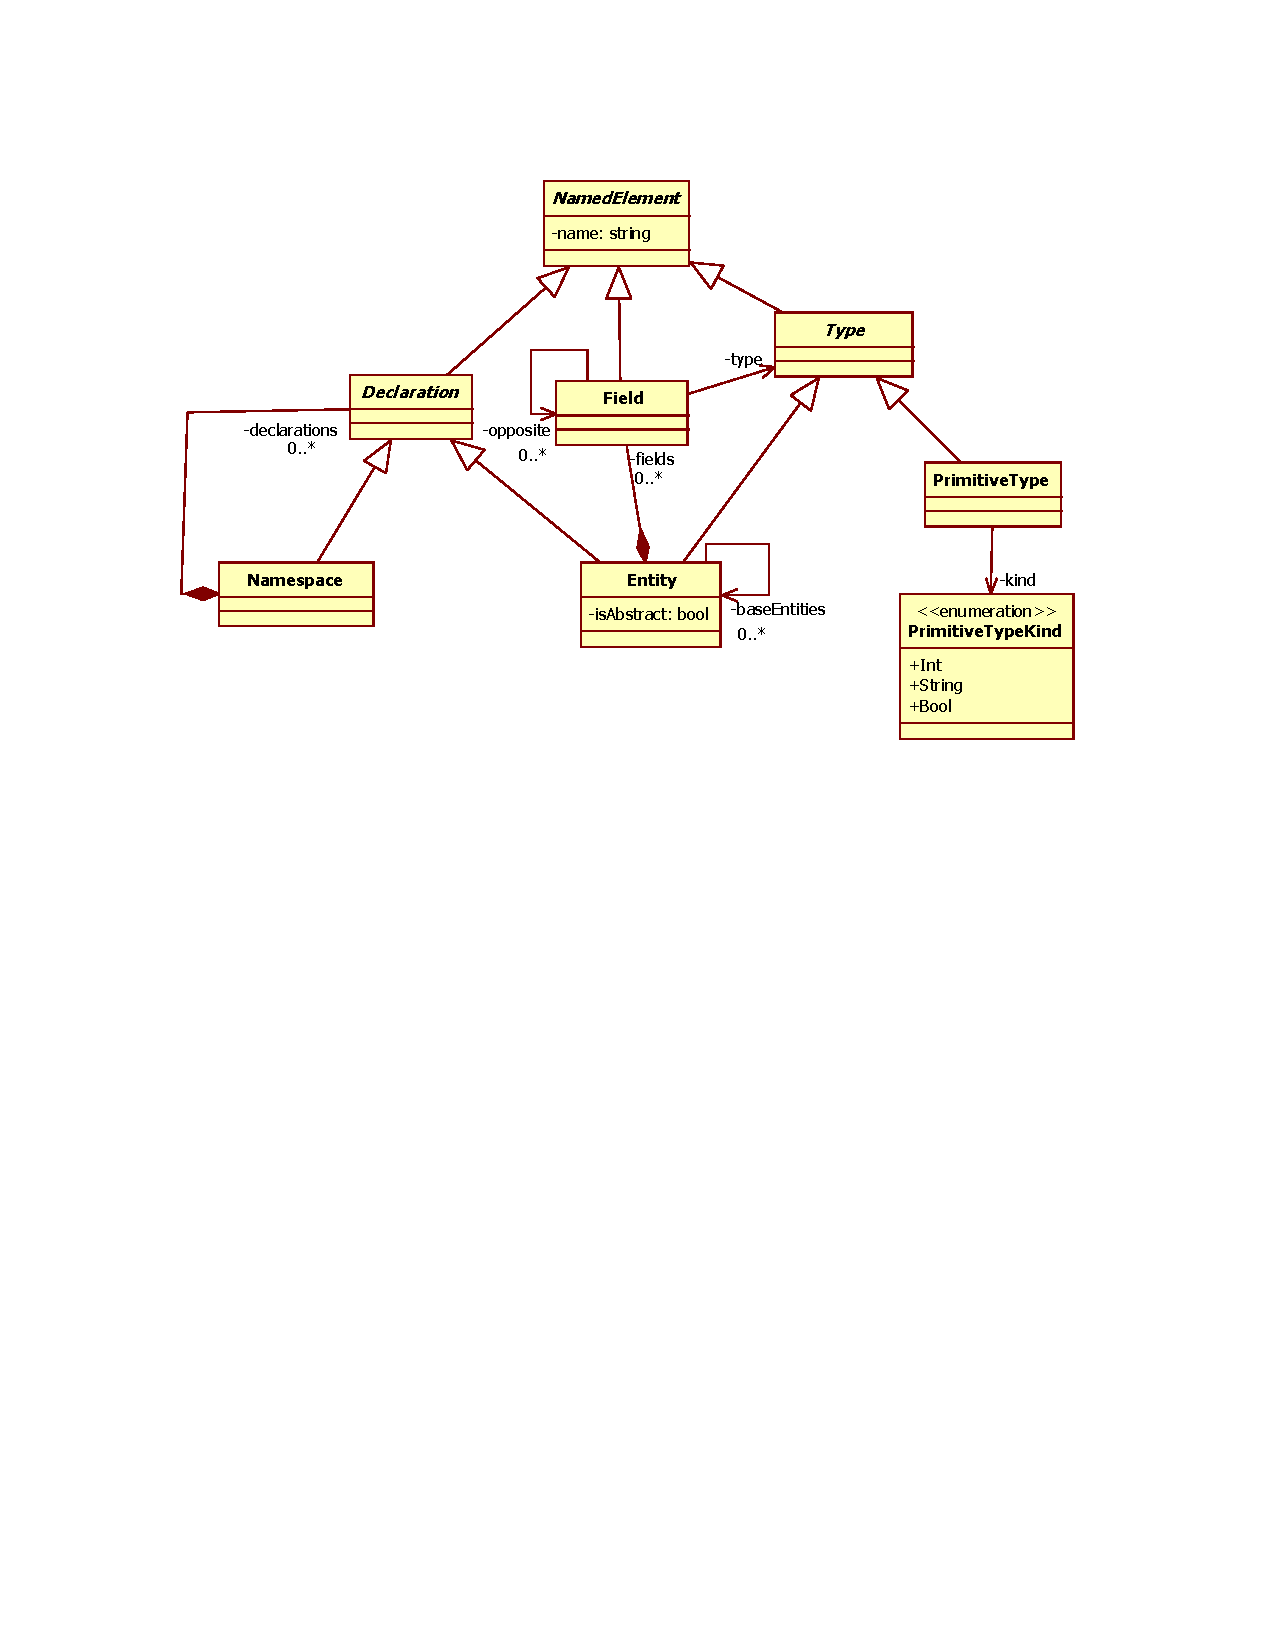
\includegraphics[trim=60 430 60 80,clip,width=\textwidth]{SampleMetaModel.pdf}\end{center}

Ennek a Meta-Model nyelven történő leírása a következő:

\metafile{sources/SampleMetaModel.mm}


A fenti metamodellnek megfelelő szöveges DSL-t fogunk készíteni, azaz definiáljuk hozzá az annotált ANTLR4 nyelvtant, amelyre építve a MetaDslx fordító a szemantikai elemzés során a metadmodellnek megfelelő modellt tud építeni. A DSL szintaktikájában nagyon hasonló lesz a fenti Meta-Model nyelv szintaxisához, a különbség csak annyi, hogy nem lesz benne \f{metamodel}, \f{enum}, \f{containment} és \f{list} kulcsszó-támogatás, és szögletes zárójelbe írt annotációk sem. A \f{class} kulcsszó helyett pedig \f{entity} kulcsszót fogunk használni. Minden más pontosan követni fogja a fenti Meta-Model szintaxist.

Például a következő kód megfelel a tervezett DSL-nek:

\metafile{sources/HusbandWifeSample.mm}

A szemantikai annotációkat a parser nyelvtani leírásába kell illeszteni, így most csak a parser nyelvtanára koncentrálunk. Az egyszerűség kedvéért az alábbi példákban a tokeneket most implicit beleírjuk a parser nyelvtanba, de ahogy az előző szakaszban említettük, a tokeneket külön lexer nyelvtanban kell definiálni és a parser nyelvtanból meg kell hivatkozni a lexer nyelvtanban definiált tokeneket.

Egy entitás szintaktikai leírását a hagyományos ANTLR4 nyelven a következőképpen kezdhetjük el megtervezni:

\begin{antlr4code}
entity: 'entity' identifier entityBody;

entityBody: '{' field* '}'
\end{antlr4code}

Az \f{entity} szabály (nemterminális) azt mondja, hogy egy entitás a kódban mindig az \f{entity} kulcsszóval kezdődik, ezt követi egy azonosító (\f{identifier}), ami az entitás neve, végül pedig az entitás törzsének leírása (\f{entityBody}) következik. Az \f{entityBody} szabály szerint az entitás törzse nyitó kapcsoszárójellel kezdődik, tetszőlegesen sok meződefiníciót (\f{field}) tartalmaz, és záró kapcsoszárójellel végződik. A \f{field} szabály a fenti példában nincs még kifejtve, de később ezt is látni fogjuk.

Ahhoz, hogy a szemantikai elemző egy \f{Entity} objektumot hozzon létre a fenti szabály hatására, a következő annotációk definiálására van szükség:

\begin{antlr4code}
$SymbolDef(Entity)
entity: 'entity' $Name identifier entityBody;

entityBody: '{' field* '}'
\end{antlr4code}

A \f{SymbolDef} annotáció jelzi, hogy amikor a szintaxisfában egy \f{entity} csúcs szerepel, annak hatására egy új modellbeli objektumot kell létrehozni. Az annotáció alapértelmezett \f{type} paramétere adja meg a létrehozandó objektum típusát.

Strukturált programnyelveknél az objektum neve valahol az objektumot definiáló csúcs részfájában szerepel. Ez azt jelenti, hogy az entitás neve közvetlenül vagy közvetve az \f{entity} szabály jobb oldalán fordul elő. Az objektum nevének helyét a \f{Name} annotációval kell jelölni, és tipikusan egy azonosítót definiáló tokenre célszerű rátenni, vagy olyan nemterminálisra, amelyből egyszerű szabályok sorozatával tokenhez jutunk. A \f{Name} annotációnak nincs paramétere, az annotáció csak jelzésértékű, hogy honnan kell kinyerni az objektum nevét.

Az objektumot definiáló csúcs részfájában a \f{Name} annotációval ellátott csúcsok száma tipikusan pontosan egy, ahogy a fenti példában is. Előfordulhat azonban, hogy több \f{Name} annotációval ellátott csúcs is van a részfában, ekkor minden egyes ilyen csúcsra egy-egy új objektum keletkezik, és mindegyik megkapja a saját nevét. Tipikus ilyen eset például, amikor C\#-ban egyetlen sorban több ugyanolyan típusú változót is definiálunk, és a nevüket vesszőkkel választjuk el. Az is előfordulhat, hogy egyetlen \f{Name} annotációval ellátott csúcs sincs az adott részfában, ekkor mindenképpen pontosan egy modellobjektum keletkezik, de névtelen, azaz anonim objektum lesz belőle. Ilyen eset tipikusan C\#-ban egy tömb típusú változó definiálása, ahol maga a tömb típus egy új anonim modellobjektum, csak a tömb elemeinek típusa egy már létező, névvel ellátott modellobjektumra történő hivatkozás.

A fentiek alapján a \f{field} szabály annotált definíciója a következő:
\begin{antlr4code}
$SymbolDef(Field)
field: typeReference $Name identifier ';';
\end{antlr4code}

Ez tehát azt jelenti, hogy egy \f{field} csúcs esetén egy új \f{Field} objektumot kell létrehozni, amelynek nevét az \f{identifier} csúcs adja.

Ha a \f{field} szabályt összevetjük a fenti \f{entity} szabály definíciójával, észrevehetjük, hogy a \f{Name} annotáció közvetve az \f{entity} részfájában is szerepel. Ez azt jelentené, hogy a mező nevével megegyező entitás is keletkezne. Ezt elkerülendő, a szabály az, hogy a \f{Name} annotáció mindig a hozzá fában felfelé legközelebbi \f{SymbolDef} annotációhoz tartozik. Strukturált programnyelvek esetén ez a kikötés mindig a helyes szemantikát adja.

A következő lépés, hogy összekössük egymással az objektumokat. Valahogy jelezni kell, hogy a létrehozott \f{Field} objektumokat a megfelelő \f{Entity} objektum alá hova kell bekötni. A metamodellben az \f{Entity}-nek a \f{Fields} nevű tulajdonsága tartalmazza az entitás mezőit, tehát ide kéne bekötni a \f{Field} objektumokat. Ezt a \f{Property} annotációval lehet elérni:

\begin{antlr4code}
$SymbolDef(Entity)
entity: 'entity' $Name identifier entityBody;

entityBody: '{' field* '}'

$Property(Fields)
$SymbolDef(Field)
field: typeReference $Name identifier ';';
\end{antlr4code}

A \f{Property} nevű szemantikai annotációval lehet értéket adni egy modellobjektum tulajdonságainak. A \f{Property} annotáció is mindig a hozzá fában felfelé legközelebbi \f{SymbolDef} annotációhoz tartozik, így fontos, hogy pontosan hova és milyen sorrendben helyezzük az annotációkat. A fenti példában a \f{field} szabály esetén a \f{\$Property(Fields)} van felül (azaz előbb), a \f{\$SymbolDef(Field)} pedig alul (azaz később). Ez azt jelzi, hogy egy új \f{Field} objektumot kell létrehozni, amelyet a felette definiált \f{Entity} objektum \f{Fields} tulajdonsága alá kell beilleszteni. Ha a sorrend fordított lenne, akkor a \f{Field} objektum \f{Fields} tulajdonságának adnánk valamilyen értéket, de neki nincs ilyen tulajdonsága.

A \f{Property} annotáció alapértelmezett \f{name} paramétere a tulajdonság nevét adja meg. A tulajdonsághoz rendelt érték több helyről is származhat. Egyik ezek közül a fenti példában is említett lehetőség: egy \f{SymbolDef} által létrehozott modellobjektumok valahol a \f{Property} annotáció részfájában.

Egy másik lehetőség a \f{Property} annotáció opcionális \f{value} paramétere, amellyel közvetlenül konkrét értéket is lehet adni az adott tulajdonságnak. Ez például az \f{abstract} kulcsszó bevezetésénél lehet hasznos:

\begin{antlr4code}
$SymbolDef(Entity)
entity: ($Property(name=IsAbstract, value=true) 'abstract')? 'entity' $Name identifier entityBody;

entityBody: '{' field* '}'
\end{antlr4code}

A fenti \f{Property} annotáció csak akkor létezik, ha az a csúcs is létezik, amihez kötődik. Itt az \f{abstract} kulcsszó opcionális, így a \f{Property} annotációnak csak akkor van hatása, ha a kódban ténylegesen szerepel az \f{abstract} kulcsszó. Ekkor az \f{Entity} objektum \f{IsAbstract} tulajdonságát igazra állítjuk a \f{Property} annotáció segítségével.

Ha a \f{value} paraméter meg van adva, akkor csak ez az érték számít a tulajdonság értékének beállításakor, a \f{Property} annotáció részfájában szereplő egyéb értékek nem.

A szemantikai elemzőnek fel kell tudnia oldani egyes modellobjektumokat a nevük alapján. Ilyenkor számít az is, hogy a feloldás helyén éppen milyen scope az érvényes. Amikor a \f{SymbolDef} annotációval egy új modellobjektumot definiálunk, akkor nem biztos, hogy az objektum minden gyereke az adott részfában egyből feloldhatóvá válik. C\#-ban például csak az osztály törzsén belül (a kapcsoszárójeleken belül) oldhatók fel az osztály törzsében definiált függvények, tulajdonságok és egyéb belső típusok. Az osztály fejlécében (pl. az ősosztályok lisájában) még nem szerepelhet olyan típus, ami az osztály törzsében van definiálva. Tehát valahol jeleznünk kell, hol lépünk be abba a scope-ba, ahol már feloldhatók a modellobjektum gyerekei is. Erre szolgál a \f{Scope} annotáció, amelyet az entitásos példánkban az entitás törzséhez kell hozzárendelni:

\begin{antlr4code}
$SymbolDef(Entity)
entity: ($Property(name=IsAbstract, value=true) 'abstract')? 'entity' $Name identifier $Scope entityBody;

entityBody: '{' field* '}'
\end{antlr4code}

Az annotációt rendelhetnénk közvetlenül az \f{entityBody} szabályhoz is:

\begin{antlr4code}
$SymbolDef(Entity)
entity: ($Property(name=IsAbstract, value=true) 'abstract')? 'entity' $Name identifier entityBody;

$Scope
entityBody: '{' field* '}'
\end{antlr4code}

A fenti két megoldás ekvivalens egymással, mert a \f{Scope} annotáció mindkét esetben az \f{entityBody} csúcshoz lesz hozzárendelve. Általánosan is igaz, hogy az annotációk köthetők a nemterminálishoz, de köthetők a szabály jobb oldalának valamelyik eleméhez is, a lényeg, hogy az elkészült szintaxisfában melyik csúcshoz milyen annotációk milyen sorrendben vannak hozzárendelve.

Ez a dinamikus játék az annotációkkal hasznos lehet a szabályok egyszerűsítésénél. Például a \f{\$Name identifier} kiszervezhető egy külön \f{name} szabályba, így a nyelvtani leírás egyszerűsödik:
\begin{antlr4code}
name: $Name identifier;
identifier: $Identifier ID;

$SymbolDef(Entity)
entity: ($Property(name=IsAbstract, value=true) 'abstract')? 'entity' name entityBody;

$Scope
entityBody: '{' field* '}'

$Property(Fields)
$SymbolDef(Field)
field: typeReference name ';';
\end{antlr4code}

Így tehát az \f{entity} és a \f{field} nevénél elég a \f{name} szabályt meghivatkozni. Egy új annotációt is találunk a fenti példában, az \f{Identifier} annotációt, amelynek segítségével a \f{Name} annotáció jelentése egy kis pontosításra szorul. Az \f{Identifier} annotáció mondja meg konkrétan azt, hogy mi lesz az objektum neve. A \f{Name} annotációt úgy kell elképzelni, hogy a hozzá tartozó csúcshoz kötődik a létrehozott modellobjektum, de az objektum nevének a tényleges értéke a \f{Name} annotáció alatti részfában az \f{Identifier} annotáció által meghatározott érték. A \f{Name} annotáció alatti részfában legalább egy \f{Identifier} annotációjú csúcsnak szerepelnie kell, különben nem jön létre objektum a \f{Name} annotáció hatására. Ha a \f{Name} annotáció alatti részfában több \f{Identifier} annotációjú csúcs is van, akkor több objektum is létrejön a megfelelő \f{Identifier} által jelzett nevekkel.

Az \f{Identifier} annotáció akkor is hasznos, ha más objektumokat a nevük alapján kell meghivatkozni. A fenti példában a \f{field} jobb oldalán a \f{typeReference} egy tipikus példája egy ilyen hivatkozásnak, ugyanis itt hivatkozunk egy másik entitásra vagy primitív típusra, amely az adott mező típusa lesz. Egy ilyen hivatkozás a \f{SymbolUse} annotációval történik, és a hivatkozott objektum nevét az alatta lévő részfában szereplő \f{Identifier} annotáció által jelzett helyről szerzi. A \f{SymbolUse} által meghivatkozott modellobjektumok is értékei lehetnek egy tulajdonságnak. A mező teljes definíciója tehát:

\begin{antlr4code}
$Property(Fields)
$SymbolDef(Field)
field: $Property(Type) typeReference name ';';

$SymbolUse(Type)
typeReference: primitiveType | identifier;

identifier: $Identifier ID;
\end{antlr4code}

A fenti példa tehát azt jelenti, hogy a \f{Field} objektum \f{Type} tulajdonságának értéke, a \f{SymbolUse} által a neve alapján feloldott modellobjektum. A \f{SymbolUse} alapértelmezett, de opcionális paramétere a \f{type}, amely annak a modellobjektumnak a típusát  (vagy őstípusát) határozza meg, amelyet fel kívánunk oldani. A \f{SymbolUse} használható paraméter nélkül is, ilyenkor bármelyik megfelelő nevű modellobjektum helyes feloldásnak tekinthető. A \f{SymbolUse} egy másik opcionális paramétere a \f{types}, itt több típus is felsorolható egyszerre, és egy megfelelő nevű modellobjektum, amelyik ezek közül bármelyik típusnak megfelel, helyes feloldásnak számít. A \f{types} paraméter értékét egyszerű kerek zárójelben vesszőkkel elválasztva kell megadni. Például a \f{\$SymbolUse(types=(Field,Namespace))} annotáció csak \f{Field} és \f{Namespace} típusú modellobjektumokat old fel.

Strukturált programnyelveknél a modellobjektumok feloldása hierarchikus névvel is történhet, tipikusan akkor, ha a hivatkozott objektum sem az aktuális scope-ban, sem annak valamely szülő scope-jában nem szerepel. Szükség van tehát arra, hogy hierarchikus azonosítót is tudjunk használni. Erre szolgál a \f{Qualifier} paraméter nélküli annotáció, amelyet a következőképpen lehet használni:

\begin{antlr4code}
$Property(Fields)
$SymbolDef(Field)
field: $Property(Type) typeReference name ';';

$SymbolUse(Type)
typeReference: primitiveType | qualifier;

$Qualifier
qualifier: identifier ('.' identifier)*;

$Identifier
identifier: ID;
\end{antlr4code}

Figyeljük meg, hogy a \f{typeReference} szabály jobb oldalán az \f{identifier}-t lecseréltük \f{qualifier}-re, és a \f{qualifier} egy hierarchikus azonosító, vagyis pontokkal elválasztott \f{identifier}-ek sorozata. A \f{qualifier} szabály megkapta a \f{Qualifier} annotációt, míg az \f{identifier} továbbra is \f{Identifier} annotációval rendelkezik. A \f{SymbolUse} annotáció részfájában tehát nem csak egyszerű \f{Identifier} annotációval rendelkező csúcsok szerepelhetnek, hanem \f{Qualifier} annotációval ellátott csúcsok is. Utóbbiak hierarchikus neveket is támogatnak a modellobjektumok név szerinti feloldása során. A hierarchiát a \f{Qualifier} alatti részfában az \f{Identifier}-ek sorrendje adja.

Mostmár az entitások közötti öröklődést is definiálhatjuk, azaz az ősentitásokra való hivatkozást:

\begin{antlr4code}
$SymbolDef(Entity)
entity: ($Property(name=IsAbstract, value=true) 'abstract')? 'entity' name (':' $Property(BaseEntities) $SymbolUse(Entity) qualifierList)? entityBody;

qualifierList: qualifier (',' qualifier)*;
\end{antlr4code}

Tehát ősentitásként tetszőleges \f{Entity} típusú objektum feloldható, és a feloldott objektumok a \f{BaseEntities} tulajdonságban tárolódnak el. A Meta-Model leírásban található \f{[BaseScope]} annotáció biztosítja, hogy a szemantikus elemzés során az ősentitásokban definiált mezők is feloldhatók. Erre szükség is lehet például az asszociációk definiálásakor:

\begin{antlr4code}
$Opposite
association: 'association' $SymbolUse(Field) source=qualifier 'with' $SymbolUse(Field) target=qualifier ';';
\end{antlr4code}

Az \f{Opposite} annotáció jelenleg nem része az itt definiált szemantikus elemzésnek, inkább csak egy példaként szolgál, hogy saját annotációk is definiálhatók, és a szemantikai elemzés ezek segítségével finomhangolható. A két asszociációban lévő mező hierarchikus azonosító alapján történő feloldását a \f{SymbolUse} miatt a szemantikai elemző automatikusan elvégzi, egyedül az \f{Opposite} tulajdonságaik beállítását kell a saját szemantikus szabályunkban megoldani. A MetaDslx keretrendszernek tehát biztosítania kell, hogy saját szemantikus szabályokat is tudjunk definiálni.

Felmerülhet a kérdés, hogy van-e értelme hierarchikus azonosítókat használni objektumok definiálásakor, vagyis a \f{Name} annotáció alatt, vagy ott csak \f{Identifier} szerepelhet? A válasz az, hogy igen, lehet értelme hierarchikus neveknek is. A saját példa DSL-ünkben ilyen a névtér definíciója, amelynél a hierarchikus név egymásba ágyazott névtereket jelent. A névter nyelvtani leírását az alábbi módon definiálhatjuk:

\begin{antlr4code}
$SymbolDef(type=Namespace,nestingProperty=Declarations,merge=true)
namespace: 'namespace' $Name qualifier namespaceBody;

$Scope
namespaceBody: '{' declaration* '}';

$Property(Declarations)
declaration: namespace | entity | association;

$Qualifier
qualifier: identifier ('.' identifier)*;

$Identifier
identifier: ID;
\end{antlr4code}

A fenti példában csak a \f{SymbolDef} annotáció két opcionális paramétere (\f{nestingProperty} és \f{merge}) az, ami újdonság, minden mást már ismerünk.

A \f{nestingProperty} paraméter a hierarchikus név miatt szükséges, ugyanis a hierarchikus név minden egyes eleme egy-egy újabb modellobjektumot (jelen esetben \f{Namespace}-t) hoz létre, amelyeket egymásba kell skatulyázni, és meg kell mondani, hogy mely tulajdonságon keresztül lehet ezt megtenni. A metamodellünkben a \f{Namespace}-ek a \f{Declarations} tulajdonságon keresztül skatulyázhatók egymásba, ezért ez az értéke ennek a paraméternek. Fontos, hogy ez a paraméter csak az egymásba skatulyázás során van figyelembe véve. A legkülső \f{Namespace} objektumot, ha valamilyen egyéb külső objektumba szeretnénk beágyazni, akkor azt a normál \f{Property} annotációval tehetjük meg, ahogy a \f{Field}-eket ágyaztuk be az \f{Entity}-kbe.

A másik érdekes új paraméter a \f{merge}. Ha ennek az értékét igazra állítjuk, akkor az azonos nevű, de ugyanolyan típusú deklarációk összevonódnak, és mindössze egyetlen modellobjektumot hoznak létre. Ez azt jelenti, hogy egy névteret ugyanolyan néven többször is definiálhatunk a kódunkban, de valójában egyetlen \f{Namespace} objektum fog hozzájuk kötődni. Az alábbi két példa tehát ekvivalens, ugyanazt a modellt hozzák létre:

\metafile{sources/HusbandWifeSample.mm}

illetve:

\metafile{sources/HusbandWifeSample2.mm}

Tehát mindegy, hogy a DSL-ünkben a névtereket hogyan daraboljuk szét, csak a három egymásba ágyazott névtér jön létre a szemantikai elemző által épített modellben.

A DSL-ünkből egyedül már csak a primitív típusok definíciója hiányzik, amelyet így lehet megtenni:

\begin{antlr4code}
primitiveType
	: $Value(PredefinedTypes.Int) 'int'
	| $Value(PredefinedTypes.String) 'string'
	| $Value(PredefinedTypes.Bool) 'bool'
	;
\end{antlr4code}

Itt a \f{Value} annotációt használjuk előre definiált értékek jelöléséhez. Ez azt jelenti, hogy a három primitív típust nem a szemantikai elemző példányosítja, hanem előre létrehozzuk, és itt már csak meghivatkozzuk őket. Ez azért hasznos, mert így elegendő ez az előre létrehozott három érték a teljes szemantikai elemzés során, nem kell belőlük sok-sok új példányt létrehozni. A \f{SymbolUse} így tehát nemcsak \f{Qualifier} vagy \f{Identifier} alapján dolgozhat, hanem előre definiált érték (\f{Value} annotáció)) alapján is.

Mostmár összerakhatjuk a DSL teljes szintaktikai és szemantikai leírását:

\begin{antlr4code}
grammar EntitySampleParser;

main: namespace* EOF;

$SymbolDef(type=Namespace,nestingProperty=Declarations,merge=true)
namespace: 'namespace' $Name qualifier namespaceBody;

$Scope
namespaceBody: '{' declaration* '}';

$Property(Declarations)
declaration: namespace | entity | association;

$SymbolDef(Entity)
entity: ($Property(name=IsAbstract, value=true) 'abstract')? 'entity' name (':' $Property(BaseEntities) $SymbolUse(Entity) qualifierList)? entityBody;

$Scope
entityBody: '{' field* '}';

$Property(Fields)
$SymbolDef(Field)
field: $Property(Type) typeReference name ';';

$SymbolUse(Type)
typeReference: primitiveType | qualifier;

primitiveType
	: $Value(PredefinedTypes.Int) 'int'
	| $Value(PredefinedTypes.String) 'string'
	| $Value(PredefinedTypes.Bool) 'bool'
	;

$Opposite
association: 'association' $SymbolUse(Field) source=qualifier 'with' $SymbolUse(Field) target=qualifier ';';

qualifierList: qualifier (',' qualifier)*;

$Name
name: identifier;

$Qualifier
qualifier: identifier ('.' identifier)*;

$Identifier
identifier: ID;

ID: [a-zA-Z_][a-zA-Z_0-9]*;
\end{antlr4code}

Ezzel a leírással a DSL-ünk szinte teljes szemantikai elemzését automatizáltan elvégezhetjük. Egyedül az asszociáció két végén lévő \f{Field} egymással való összekötése hiányzik, de a két vég feloldását a szemantikai elemző automatikusan megoldja. Jól látható tehát, hogy a szemantikai elemzésből nagyon sokminden általánosítható. Az elsődleges cél az itt definiált annotációk támogatása. Távolabbi cél a még részletesebb szemantikai elemzés, például a kifejezések automatikus szemantikai elemzése. Ez is egy jól általánosítható terület, hiszen nagyon sok nyelvben egymáshoz nagyon hasonló kifejezéseket lehet írni (pl. matematikai műveletek, függvényhívások, stb.)


\chapter{Összefoglalás}

Ez a dokumentum a MetaDslx keretrendszer elemeinek használatát mutatta be. A Meta-Model nyelv (.mm) metamodellek leírására szolgál egyszerű szöveges osztálydiagram-jellegű nyelven. A Meta-Generator nyelv (.mgen) kódgenerátorok leírását támogatja egyszerű szöveges sablon alapú nyelven. Az Annotált ANTLR4 nyelv (.ag4) fordítóprogramok definiálására szolgál annotációkkal kiegészített ANTLR4 nyelven.

\bibliographystyle{ieeetr}
\bibliography{references}

\end{document}          
